% ============================================
% DEMODULAÇÃO FM E PLL
% ============================================

\section{Demodulação FM}

\begin{frame}{Demodular FM: frequência vira amplitude}

\small
\begin{columns}[T]
\column{0.4\textwidth}
Objetivo: recuperar $m(t)$ de
\[
s(t) = A_c\cos[2\pi f_c t + \phi(t)]
\]

\onslide<2->{Ideia comum: um sistema cujo ganho cresce com a frequência transforma $f_i(t)$ em amplitude.}

\onslide<4->{Caminhos que veremos:
\begin{itemize}\itemsep0pt
\item derivador e detector de envoltória;
\item flanco de um ressonante, simples e balanceado;
\item demodulador coerente de NBFM;
\item PLL, na próxima seção.
\end{itemize}}

\column{0.6\textwidth}
\centering
\begin{tikzpicture}[scale=0.85, >={Stealth}]
\draw[->] (0,0) -- (5,0) node[right, font=\scriptsize] {$f$};
\draw[->] (0,0) -- (0,2.6) node[above, font=\scriptsize] {$|H(f)|$};
\draw[very thick, cBlue] (0.5,0.25) -- (4.5,2.25);
\draw[dashed, gray] (2.5,0) -- (2.5,1.25) -- (0,1.25);
\node[font=\scriptsize, below] at (2.5,-0.05) {};
\onslide<2->{
  \fill[cGreen, opacity=0.15] (1.7,0) rectangle (3.3,2.5);
  \draw[cGreen, very thick, domain=0:2, samples=80, smooth] plot ({2.5+0.8*sin(deg(2*pi*\x))}, {-0.25-1.0*\x});
  \draw[->, gray] (5.3,-0.25) -- (5.3,-2.4) node[below, font=\tiny] {$t$};
  \node[font=\scriptsize, cGreen, anchor=east] at (1.6,-1.2) {$f_i(t)$};
  \node[font=\tiny, anchor=north] at (2.5,-2.3) {$f_c$};}
\onslide<3->{
  \draw[dashed, cRed] (1.7,0) -- (1.7,0.85) -- (5.2,0.85);
  \draw[dashed, cRed] (3.3,0) -- (3.3,1.65) -- (5.2,1.65);
  \draw[cRed, very thick, domain=0:2, samples=80, smooth] plot ({5.4+1.3*\x}, {1.25+0.4*cos(deg(2*pi*\x))});
  \draw[->, gray] (5.4,0.4) -- (8.2,0.4) node[right, font=\tiny] {$t$};
  \node[font=\scriptsize, cRed, anchor=south] at (6.7,1.7) {amplitude};}
\end{tikzpicture}
\end{columns}

\end{frame}

% ============================================

\begin{frame}{Discriminador: derivador e envoltória}

\small\compacto
\begin{columns}[T]
\column{0.5\textwidth}
\centering
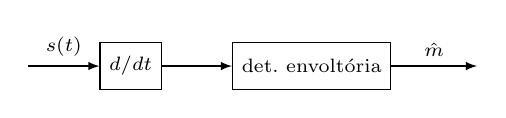
\begin{tikzpicture}[>=latex, font=\scriptsize]
\node[draw, minimum height=0.6cm] (der) at (0,0) {$d/dt$};
\node[draw, minimum height=0.6cm, align=center] (env) at (2.3,0) {det.\ envoltória};
\draw[->] (-1.3,0) -- node[above] {$s(t)$} (der);
\draw[->] (der) -- (env);
\draw[->] (env) -- node[above] {$\hat m$} (4.4,0);
\end{tikzpicture}

\raggedright
\vspace{0.1cm}
\onslide<2->{\[
\frac{ds}{dt} = -A_c\,\tikzmarknode{dth}{\big[2\pi f_c + \dot\phi(t)\big]}\sin[2\pi f_c t + \phi(t)]
\]}

\vspace{0.45cm}
\onslide<3->{Como $\dot\phi = 2\pi k_f m(t)$, a envoltória é
\[
A(t) = 2\pi A_c f_i(t) = 2\pi A_c f_c\Big[1 + \tikzmarknode{rz}{\frac{k_f m(t)}{f_c}}\Big]
\]}

\vspace{0.35cm}
\onslide<4->{Tirando o nível DC: $\hat m(t) \propto m(t)$.}

\column{0.5\textwidth}
\begin{tikzpicture}
\pgfplotsset{p/.style={onda, width=6cm, height=0.75cm, domain=0:2, samples=500}}
\begin{axis}[p, ymin=-1.3, ymax=1.3, ylabel={$s(t)$}]
\addplot[cBlue] {cos(deg(2*pi*6*x + 3*sin(deg(2*pi*x))))};
\end{axis}
\onslide<2->{
\begin{axis}[p, ymin=-1.3, ymax=1.3, ylabel={$ds/dt$}, at={(0,-1.35cm)}]
\addplot[cRed] {-(6+3*cos(deg(2*pi*x)))/9*sin(deg(2*pi*6*x + 3*sin(deg(2*pi*x))))};
\only<3->{\addplot[cRed!50!black, thick, dashed] {(6+3*cos(deg(2*pi*x)))/9};}
\end{axis}}
\onslide<4->{
\begin{axis}[p, ymin=-1.3, ymax=1.3, ylabel={$\hat m(t)$}, at={(0,-2.7cm)}]
\addplot[cGreen, very thick] {cos(deg(2*pi*x))};
\end{axis}}
\end{tikzpicture}

{\scriptsize $f_c$ baixo, só para enxergar: aqui $\Delta f/f_c = 50\,\%$.}
\end{columns}

\only<2->{\anotacoes{
  \node[nota=cRed, anchor=north] (a1) at ([yshift=-0.25cm]dth.south) {regra da cadeia: $\dot\theta = 2\pi f_i$};
  \draw[setinha, cRed] (a1.north) -- (dth.south);
}}
\only<3->{\anotacoes{
  \node[nota=cPurple, anchor=north] (a2) at ([yshift=-0.25cm]rz.south) {FM comercial: $75\,\text{kHz}/100\,\text{MHz} = 0{,}08\,\%$};
  \draw[setinha, cPurple] (a2.north) -- (rz.south);
}}

\end{frame}

% ============================================

\begin{frame}{Ruído de amplitude contamina a saída}

\small\compacto
\begin{columns}[T]
\column{0.48\textwidth}
O canal faz a amplitude variar:
\[
\rule{0pt}{0.8cm}r(t) = \tikzmarknode{At}{A(t)}\cos\theta(t)
\]

\onslide<2->{\[
\frac{dr}{dt} = \tikzmarknode{dA}{\dot A\cos\theta} - A(t)\,2\pi f_i(t)\sin\theta
\]}

\vspace{0.4cm}
\onslide<3->{A envoltória da derivada fica $A(t)\cdot 2\pi f_i(t)$: a variação de $A(t)$ entra na saída como se fosse mensagem.}

\vspace{0.1cm}
\onslide<4->{Solução: deixar a amplitude constante antes do discriminador. Em FM, a informação está só na frequência.}

\column{0.52\textwidth}
\begin{tikzpicture}
\pgfplotsset{p/.style={onda, width=6.2cm, height=0.9cm, domain=0:2, samples=500}}
\begin{axis}[p, ymin=-1.6, ymax=1.6, ylabel={$r(t)$}]
\addplot[cBlue] {(1+0.4*sin(deg(2*pi*0.7*x+1)))*cos(deg(2*pi*6*x + 3*sin(deg(2*pi*x))))};
\addplot[cOrange, dashed, thick] {1+0.4*sin(deg(2*pi*0.7*x+1))};
\end{axis}
\onslide<3->{
\begin{axis}[p, ymin=-0.1, ymax=1.5, ylabel={envoltória de $dr/dt$}, at={(0,-1.7cm)}]
\addplot[cGreen, dashed] {(6+3*cos(deg(2*pi*x)))/9};
\addplot[cRed, very thick] {(1+0.4*sin(deg(2*pi*0.7*x+1)))*(6+3*cos(deg(2*pi*x)))/9};
\end{axis}}
\end{tikzpicture}

\onslide<3->{\scriptsize \textcolor{cGreen}{tracejado: o que queríamos}, \textcolor{cRed}{cheio: o que sai}.}
\end{columns}

\only<2->{\anotacoes{
  \node[nota=cOrange, anchor=south] (a1) at ([yshift=0.12cm]At.north) {desvanecimento, ruído};
  \draw[setinha, cOrange] (a1.south) -- (At.north);
  \node[font=\scriptsize, text=gray, anchor=north] (a2) at ([yshift=-0.2cm]dA.south) {lento: pequeno};
}}

\end{frame}

% ============================================

\begin{frame}{Limitador de amplitude}

\small
\centering
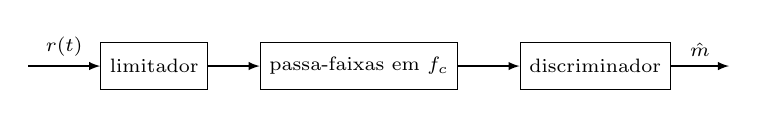
\begin{tikzpicture}[>=latex, font=\scriptsize]
\node[draw, minimum height=0.6cm] (lim) at (0,0) {limitador};
\node[draw, minimum height=0.6cm] (bpf) at (2.6,0) {passa-faixas em $f_c$};
\node[draw, minimum height=0.6cm] (dis) at (5.6,0) {discriminador};
\draw[->] (-1.6,0) -- node[above] {$r(t)$} (lim);
\draw[->] (lim) -- (bpf);
\draw[->] (bpf) -- (dis);
\draw[->] (dis) -- node[above] {$\hat m$} (7.3,0);
\end{tikzpicture}

\vspace{0.15cm}
\begin{columns}[T]
\column{0.3\textwidth}
\centering
\begin{tikzpicture}
\begin{axis}[espec, axis lines=middle, width=2.8cm, height=2.4cm, xmin=-1.2, xmax=1.2, ymin=-1.3, ymax=1.3,
             xtick=\empty, ytick={-1,1}, yticklabels={$-V$, $V$}, xlabel={entrada}, ylabel={saída}]
\addplot[very thick, cPurple, domain=-1.2:1.2, samples=100] {max(-1, min(1, 6*x))};
\end{axis}
\end{tikzpicture}

{\scriptsize Satura em $\pm V$ para quase toda a entrada.}

\column{0.7\textwidth}
\begin{tikzpicture}
\pgfplotsset{p/.style={onda, width=8cm, height=0.75cm, domain=0:2, samples=700}}
\begin{axis}[p, ymin=-1.6, ymax=1.6, ylabel={$r(t)$}]
\addplot[cBlue] {(1+0.4*sin(deg(2*pi*0.7*x+1)))*cos(deg(2*pi*6*x + 3*sin(deg(2*pi*x))))};
\end{axis}
\onslide<2->{
\begin{axis}[p, ymin=-1.6, ymax=1.6, ylabel={limitado}, at={(0,-1.3cm)}]
\addplot[cPurple] {max(-1, min(1, 6*(1+0.4*sin(deg(2*pi*0.7*x+1)))*cos(deg(2*pi*6*x + 3*sin(deg(2*pi*x))))))};
\end{axis}}
\onslide<3->{
\begin{axis}[p, ymin=-1.6, ymax=1.6, ylabel={após filtro}, at={(0,-2.6cm)}]
\addplot[cGreen] {1.27*cos(deg(2*pi*6*x + 3*sin(deg(2*pi*x))))};
\addplot[cGreen!50!black, dashed] {1.27};
\end{axis}}
\end{tikzpicture}
\end{columns}

\vspace{0.1cm}
\raggedright
\onslide<2->{O limitador entrega uma onda quase quadrada: mesmos cruzamentos por zero, amplitude fixa.}
\onslide<3->{O passa-faixas fica com a fundamental, de amplitude $4V/\pi$, constante.}

\end{frame}

% ============================================

\begin{frame}{Derivador como filtro linear}

\small\compacto
\begin{columns}[T]
\column{0.45\textwidth}
No tempo, $y(t) = ds/dt$. Na frequência:
\[
Y(f) = j2\pi f\, S(f) \;\Rightarrow\; \boxed{\,|H_d(f)| = 2\pi|f|\,}
\]

\vspace{0.1cm}
\onslide<2->{O FM ocupa só $f_c \pm B_T/2$.}

\vspace{0.1cm}
\onslide<3->{Ampliando essa janela, o ganho quase não muda: varia $\pm\Delta f/f_c$.}

\vspace{0.1cm}
\onslide<4->{A mensagem é essa pequena inclinação sobre um nível DC grande, $2\pi f_c$.}

\column{0.55\textwidth}
\begin{tikzpicture}
\begin{axis}[espec, axis lines=middle, width=5.4cm, height=1.9cm, xmin=-1.3, xmax=1.3, ymin=0, ymax=1.35,
             xtick={-1,1}, xticklabels={$-f_c$, $f_c$}, ytick=\empty, xlabel={$f$}, ylabel={$|H_d(f)|$}]
\addplot[very thick, cBlue, domain=-1.25:1.25] {abs(x)};
\onslide<2->{\fill[cGreen, opacity=0.3] (axis cs:0.95,0) rectangle (axis cs:1.05,1.3);
  \fill[cGreen, opacity=0.3] (axis cs:-1.05,0) rectangle (axis cs:-0.95,1.3);}
\onslide<3->{\draw[cRed, thick] (axis cs:0.9,0.85) rectangle (axis cs:1.1,1.15);}
\end{axis}
\onslide<3->{
\begin{axis}[espec, width=5.4cm, height=1.5cm, xmin=-3, xmax=3, ymin=0, ymax=1.2, at={(0,-2.8cm)},
             xtick={-1,0,1}, xticklabels={$f_c{-}\Delta f$, $f_c$, $f_c{+}\Delta f$}, ytick={1}, yticklabels={$2\pi f_c$},
             xlabel={}, ylabel={zoom}]
\fill[cGreen, opacity=0.15] (axis cs:-1,0) rectangle (axis cs:1,1.2);
\addplot[very thick, cBlue, domain=-3:3] {1 + 0.02*x};
\end{axis}
\draw[cRed, ->] (4.5,0.2) to[bend left=20] (4.2,-0.9);}
\end{tikzpicture}
\end{columns}

\end{frame}

% ============================================

\begin{frame}{Por que não um derivador de verdade?}

\small
\begin{columns}[T]
\column{0.45\textwidth}
Basta o filtro ser linear dentro de $B_T$ em torno de $f_c$:
\[
|H(f_c + \delta)| \approx a_0 + a_1\delta
\]

\onslide<2->{O derivador exato tem ganho que cresce sem limite e amplifica o ruído fora da banda.}

\vspace{0.15cm}
\onslide<3->{E não se realiza com componentes passivos em toda a faixa.}

\vspace{0.15cm}
\onslide<4->{Solução: um passa-faixas cujo flanco imita a rampa só dentro de $B_T$.}

\column{0.55\textwidth}
\begin{tikzpicture}
\begin{axis}[espec, width=5.6cm, height=3.3cm, xmin=0, xmax=2.2, ymin=0, ymax=1.35,
             xtick={1}, xticklabels={$f_c$}, ytick=\empty, xlabel={$f$}, ylabel={ganho}]
\fill[cGreen, opacity=0.15] (axis cs:0.9,0) rectangle (axis cs:1.1,1.35);
\addplot[very thick, cBlue, domain=0:2.2] {0.55*x};
\onslide<2->{\fill[cRed, opacity=0.1] (axis cs:1.3,0) rectangle (axis cs:2.2,1.35);
  \node[font=\tiny, cRed, align=center] at (axis cs:1.75,1.2) {ruído\\ amplificado};}
\onslide<4->{\addplot[very thick, cOrange, domain=0.3:2.2, samples=200] {0.8/sqrt(1+(4*(x-1.18))^2)};
  \node[font=\tiny, cOrange] at (axis cs:1.62,0.42) {passa-faixas};}
\end{axis}
\end{tikzpicture}
\end{columns}

\end{frame}

% ============================================

\begin{frame}{Slope detector com ressonante}

\small\compacto
\begin{columns}[T]
\column{0.44\textwidth}
Tanque $LC$ com fator $Q$ e ressonância $f_0$:
\[
|H(f)| = \frac{1}{\sqrt{1 + Q^2\big(\frac{f}{f_0} - \frac{f_0}{f}\big)^2}}
\]

\onslide<2->{Sintonizamos $f_0$ ao lado de $f_c$: a portadora cai no flanco.}

\vspace{0.15cm}
\onslide<3->{Cada valor de $f_i(t)$ dá um ganho diferente.}

\vspace{0.15cm}
\onslide<6->{Perto de $f_c$, o flanco é quase a rampa do derivador.}

\column{0.56\textwidth}
\begin{tikzpicture}
\begin{axis}[espec, width=5.8cm, height=3.4cm, xmin=180, xmax=230, ymin=0, ymax=1.1,
             xtick={200,206}, xticklabels={$f_c$, $f_0$},
             x tick label style={font=\tiny}, ytick={0.5,1}, xlabel={$f$ [kHz]}, ylabel={$|H(f)|$}]
\addplot[very thick, cBlue, domain=180:230, samples=200] {1/sqrt(1+400*(x/206-206/x)^2)};
\onslide<2->{\fill[cGreen, opacity=0.15] (axis cs:196,0) rectangle (axis cs:204,1.1);}
\only<3>{\draw[cRed, dashed, thick] (axis cs:196,0) -- (axis cs:196,0.449) -- (axis cs:180,0.449);
  \fill[cRed] (axis cs:196,0.449) circle (1.8pt);}
\only<4>{\draw[cRed, dashed, thick] (axis cs:200,0) -- (axis cs:200,0.646) -- (axis cs:180,0.646);
  \fill[cRed] (axis cs:200,0.646) circle (1.8pt);}
\only<5->{\draw[cRed, dashed, thick] (axis cs:204,0) -- (axis cs:204,0.932) -- (axis cs:180,0.932);
  \fill[cRed] (axis cs:204,0.932) circle (1.8pt);}
\onslide<6->{\addplot[cOrange, very thick, domain=193:207] {0.646 + 0.0605*(x-200)};}
\end{axis}
\end{tikzpicture}

{\scriptsize $f_c = 200$ kHz, $f_0 = 206$ kHz, $Q = 20$.}
\end{columns}

\end{frame}

% ============================================

\begin{frame}{Derivador versus flanco}

\small
$f_c = 200$\,kHz, $\Delta f = 4$\,kHz, $f_m = 1$\,kHz; tudo normalizado pelo valor em $f_c$.

\vspace{0.1cm}
\centering
\begin{tikzpicture}
\pgfplotsset{h/.style={espec, width=5cm, height=1.15cm, xmin=180, xmax=220, ymin=0, ymax=1.8,
             xtick={190,200,210}, ytick={1}, xlabel={$f$ [kHz]}},
             e/.style={espec, width=5cm, height=1.15cm, xmin=0, xmax=3, ymin=0, ymax=1.8, domain=0:3, samples=200,
             xtick={1,2,3}, ytick={1}, xlabel={$t$ [ms]}}}
\begin{axis}[h, ylabel={derivador}]
\fill[cGreen, opacity=0.15] (axis cs:196,0) rectangle (axis cs:204,1.8);
\addplot[very thick, cBlue, domain=180:220] {x/200};
\end{axis}
\onslide<2->{
\begin{axis}[e, at={(6.6cm,0)}, ylabel={envoltória}]
\addplot[very thick, cBlue] {1 + 0.02*cos(deg(2*pi*x))};
\node[nota=cBlue, anchor=south] at (axis cs:1.5,1.15) {$\pm 2\,\%$};
\end{axis}}
\onslide<3->{
\begin{axis}[h, at={(0,-2.0cm)}, ylabel={flanco}]
\fill[cRed, opacity=0.12] (axis cs:196,0) rectangle (axis cs:204,1.8);
\addplot[very thick, cRed, domain=180:220, samples=200] {1/sqrt(1+400*(x/206-206/x)^2)/0.6456};
\end{axis}}
\onslide<4->{
\begin{axis}[e, at={(6.6cm,-2.0cm)}, ylabel={envoltória}]
\addplot[very thick, cRed] {1/sqrt(1+400*((200+4*cos(deg(2*pi*x)))/206-206/(200+4*cos(deg(2*pi*x))))^2)/0.6456};
\node[nota=cRed, anchor=south] at (axis cs:1.5,1.5) {$+44\,\%$ e $-30\,\%$};
\end{axis}}
\end{tikzpicture}

\raggedright
\onslide<5->{O derivador puro varia só $\Delta f/f_c = 2\,\%$. No flanco, a mesma excursão percorre a parte íngreme de $|H(f)|$.}

\end{frame}

% ============================================

\begin{frame}{Slope detector: linearidade}

\small\compacto
\begin{columns}[T]
\column{0.5\textwidth}
Taylor de $|H|$ em torno de $f_c$:
\[
|H(f_c + \delta)| = a_0 + \tikzmarknode{a1}{a_1\delta} + \tikzmarknode{a2}{a_2\delta^2} + a_3\delta^3 + \cdots
\]

\vspace{0.5cm}
\onslide<3->{Com $\delta = k_f m(t)$ e sem o nível DC:
\[
\hat m \propto a_1 k_f m + a_2 k_f^2 m^2 + a_3 k_f^3 m^3 + \cdots
\]}

\onslide<4->{Com um tom, $m^2 = \tfrac12 + \tfrac12\cos 2\omega_m t$: aparece o segundo harmônico.}

\vspace{0.1cm}
\onslide<5->{Filtro único: $a_2 \neq 0$. Só fica fiel se $|m|$ for pequeno.}

\column{0.5\textwidth}
\begin{tikzpicture}
\begin{axis}[espec, width=5.2cm, height=1.8cm, xmin=-1.3, xmax=1.3, ymin=0.4, ymax=1.0, axis lines=left,
             xtick={-1,0,1}, xticklabels={$-\Delta f$, $0$, $\Delta f$}, ytick=\empty, xlabel={$\delta$}, ylabel={$|H|$}]
\addplot[very thick, cBlue, domain=-1.3:1.3, samples=100] {1/sqrt(1+(-1+0.3*x)^2)};
\onslide<2->{\addplot[cOrange, thick, dashed, domain=-1.3:1.3] {0.7071 + 0.3*0.3536*x};
  \fill[cRed, opacity=0.25, domain=-1.3:1.3, samples=60] plot (\x, {1/sqrt(1+(-1+0.3*\x)^2)}) -- plot[domain=1.3:-1.3] (\x, {0.7071 + 0.3*0.3536*\x}) -- cycle;}
\end{axis}
\onslide<4->{
\begin{axis}[onda, width=5.2cm, height=1.1cm, domain=0:2, samples=200, ymin=-1.5, ymax=1.5, ylabel={$\hat m(t)$}, at={(0,-2.4cm)}]
\addplot[cGreen, dashed] {cos(deg(2*pi*x))};
\addplot[cRed, very thick] {cos(deg(2*pi*x)) + 0.35*cos(deg(2*pi*x))^2 - 0.175};
\end{axis}}
\end{tikzpicture}

\onslide<4->{\scriptsize \textcolor{cGreen}{ideal} e \textcolor{cRed}{com $a_2$}, exagerado: picos desiguais.}
\end{columns}

\only<2>{\anotacoes{
  \node[nota=cOrange, anchor=north] (n1) at ([xshift=-0.5cm, yshift=-0.3cm]a1.south) {reta tangente};
  \draw[setinha, cOrange] (n1.north) -- (a1.south);
  \node[nota=cRed, anchor=north] (n2) at ([xshift=0.6cm, yshift=-0.3cm]a2.south) {curvatura: distorção};
  \draw[setinha, cRed] (n2.north) -- (a2.south);
}}

\end{frame}

% ============================================

\begin{frame}{Slope detector balanceado}

\small
\begin{columns}[T]
\column{0.42\textwidth}
\onslide<1->{Dois ressonantes, um acima e outro abaixo de $f_c$, à mesma distância.}

\vspace{0.15cm}
\onslide<3->{Subtraindo as envoltórias:
\[
H_{\text{bal}}(f) = |H_1(f)| - |H_2(f)|
\]}

\onslide<4->{Curva em S, ímpar em torno de $f_c$: passa por zero em $f_c$ e é bem mais reta que cada flanco.}

\vspace{0.1cm}
\onslide<5->{Os termos pares de Taylor se cancelam. Os próximos slides mostram por quê.}

\column{0.58\textwidth}
\begin{tikzpicture}
\begin{axis}[espec, axis lines=middle, width=6.2cm, height=3.6cm, xmin=-4, xmax=4, ymin=-0.85, ymax=1.15,
             xtick={-1,1}, xticklabels={$f_c{-}W$, $f_c{+}W$}, ytick=\empty, xlabel={$f$}]
\addplot[thick, cBlue, domain=-4:4, samples=150] {1/sqrt(1+(x-1)^2)};
\node[font=\scriptsize, cBlue] at (axis cs:1.9,1.0) {$|H_1|$};
\onslide<2->{\addplot[thick, cRed, domain=-4:4, samples=150] {1/sqrt(1+(x+1)^2)};
  \node[font=\scriptsize, cRed] at (axis cs:-1.9,1.0) {$|H_2|$};}
\onslide<4->{\fill[cGreen, opacity=0.15] (axis cs:-0.6,-0.85) rectangle (axis cs:0.6,1.15);
  \addplot[very thick, cPurple, domain=-4:4, samples=200] {1/sqrt(1+(x-1)^2) - 1/sqrt(1+(x+1)^2)};
  \node[font=\scriptsize, cPurple] at (axis cs:2.9,0.42) {$H_{\text{bal}}$};}
\end{axis}
\end{tikzpicture}
\end{columns}

\end{frame}

% ============================================

\begin{frame}{Só os termos ímpares -- I}

\small\compacto
\begin{columns}[T]
\column{0.56\textwidth}
Simetria especular:
\[
|H_2(f_c + \delta)| = |H_1(f_c - \delta)|
\]

\onslide<2->{Taylor de $|H_1|$ em $f_c$:
\[
|H_1(f_c + u)| = a_0 + a_1 u + a_2 u^2 + a_3 u^3 + \cdots
\]}

\onslide<3->{Em $u = -\delta$, cada potência vira $\tikzmarknode{pot}{(-\delta)^n = (-1)^n\delta^n}$:
\[
|H_2(f_c + \delta)| = a_0 \tikzmarknode{imp}{- a_1\delta} + a_2\delta^2 - a_3\delta^3 + \cdots
\]}

\column{0.44\textwidth}
\begin{tikzpicture}
\begin{axis}[espec, axis lines=middle, width=4.6cm, height=3.2cm, xmin=-2.6, xmax=2.6, ymin=0, ymax=1.1,
             xtick={0}, xticklabels={$f_c$}, ytick=\empty, xlabel={$\delta$}]
\addplot[thick, cBlue, domain=-2.6:2.6, samples=120] {1/sqrt(1+(x-1)^2)};
\node[font=\scriptsize, cBlue] at (axis cs:1.6,1.02) {$|H_1|$};
\onslide<1->{\addplot[thick, cRed, dashed, domain=-2.6:2.6, samples=120] {1/sqrt(1+(x+1)^2)};
  \node[font=\scriptsize, cRed] at (axis cs:-1.6,1.02) {$|H_2|$};}
\onslide<3->{\draw[gray, <->] (axis cs:-0.8,0.25) -- (axis cs:0.8,0.25) node[midway, below, font=\tiny] {espelho};}
\end{axis}
\end{tikzpicture}
\end{columns}

\only<4->{\anotacoes{
  \node[nota=cRed, anchor=north] (n1) at ([yshift=-0.3cm]imp.south) {ímpares trocam de sinal; pares, não};
  \draw[setinha, cRed] (n1.north) -- (imp.south);
}}

\end{frame}

% ============================================

\begin{frame}{Só os termos ímpares -- II}

\small\compacto
\begin{columns}[T]
\column{0.56\textwidth}
Subtraindo termo a termo:
\[
H_{\text{bal}}(f_c + \delta) = \sum_{n \ge 0} a_n\,\tikzmarknode{fat}{\big[1 - (-1)^n\big]}\,\delta^n
\]

\vspace{0.35cm}
\onslide<2->{$n$ par: $1 - 1 = 0$, cancela. \quad $n$ ímpar: $1 + 1 = 2$, dobra.}

\onslide<3->{\[
\boxed{\,H_{\text{bal}}(f_c + \delta) = 2a_1\delta + 2a_3\delta^3 + 2a_5\delta^5 + \cdots\,}
\]}


\column{0.44\textwidth}
\begin{tikzpicture}
\begin{axis}[espec, axis lines=middle, width=4.6cm, height=2.6cm, xmin=-2.2, xmax=2.2, ymin=-0.9, ymax=0.9,
             xtick=\empty, ytick=\empty, xlabel={$\delta$}]
\onslide<3->{\addplot[thick, cOrange, dashed, domain=-2.2:2.2] {0.7071*x};
  \node[font=\tiny, cOrange, anchor=west] at (axis cs:0.9,0.75) {$2a_1\delta$};}
\addplot[very thick, cPurple, domain=-2.2:2.2, samples=150] {1/sqrt(1+(x-1)^2) - 1/sqrt(1+(x+1)^2)};
\node[font=\scriptsize, cPurple, anchor=north west] at (axis cs:0.6,0.3) {$H_{\text{bal}}$};
\end{axis}
\end{tikzpicture}

\onslide<4->{\scriptsize Perto de $f_c$ a curva cola na reta: o erro começa em $\delta^3$.}
\end{columns}

\only<1->{\anotacoes{
  \node[nota=cRed, anchor=north] (n1) at ([yshift=-0.3cm]fat.south) {$0$ ou $2$};
  \draw[setinha, cRed] (n1.north) -- (fat.south);
}}

\end{frame}

% ============================================

\begin{frame}{Do fator $Q$ para a variável $x$}

\small\compacto
\begin{columns}[T]
\column{0.58\textwidth}
\only<1-4>{Partimos do tanque $LC$:
\[
|H(f)| = \frac{1}{\sqrt{1 + Q^2\big(\frac{f}{f_0} - \frac{f_0}{f}\big)^2}}
\]

\onslide<2->{Denominador comum no termo entre parênteses:
\[
Q\Big(\frac{f}{f_0} - \frac{f_0}{f}\Big) = Q\,\frac{f^2 - f_0^2}{f f_0}
= Q\,\frac{(f - f_0)\tikzmarknode{soma}{(f + f_0)}}{\tikzmarknode{prod}{f f_0}}
\]}

\vspace{0.6cm}
\onslide<3->{Perto da ressonância, $f \approx f_0$:
\[
Q\,\frac{(f - f_0)\,2f_0}{f_0^2} = \tikzmarknode{xx}{\frac{f - f_0}{f_0/(2Q)}}
\]}}%
\only<5->{Perto de $f_0$, o termo $Q\big(\frac{f}{f_0} - \frac{f_0}{f}\big)$ vira $\dfrac{f - f_0}{W}$, com $W = \dfrac{f_0}{2Q}$.

\vspace{0.3cm}
Logo:
\[
\boxed{\,|H(f)| = \frac{1}{\sqrt{1 + x^2}},\quad x = \frac{f - f_0}{W}\,}
\]

\vspace{0.2cm}
Esse é o modelo usado no exemplo a seguir.}

\column{0.42\textwidth}
\onslide<5->{\begin{tikzpicture}
\begin{axis}[espec, width=4.5cm, height=3.0cm, xmin=0.6, xmax=1.4, ymin=0, ymax=1.1,
             xtick={0.9,1,1.1}, xticklabels={$-W$, $f_0$, $W$}, ytick={0.707,1}, yticklabels={$1/\sqrt2$, $1$},
             xlabel={$f$}, ylabel={$|H|$}]
\addplot[very thick, cBlue, domain=0.6:1.4, samples=200] {1/sqrt(1+25*(x-1/x)^2)};
\addplot[thick, cOrange, dashed, domain=0.6:1.4, samples=200] {1/sqrt(1+((x-1)/0.1)^2)};
\draw[dashed, gray] (axis cs:0.9,0) -- (axis cs:0.9,0.707) -- (axis cs:1.1,0.707) -- (axis cs:1.1,0);
\node[font=\tiny, cBlue, anchor=west] at (axis cs:1.15,0.75) {exata, $Q = 5$};
\node[font=\tiny, cOrange, anchor=west] at (axis cs:1.15,0.6) {em $x$};
\end{axis}
\end{tikzpicture}

\scriptsize Em $x = \pm1$ o ganho cai a $1/\sqrt2$: $W$ é a meia largura de $-3$\,dB e $2W = f_0/Q$.}
\end{columns}

\only<3-4>{\anotacoes{
  \node[nota=cRed, anchor=north east] (n1) at ([xshift=-0.2cm, yshift=-0.2cm]soma.south) {$f + f_0 \approx 2f_0$};
  \draw[setinha, cRed] (n1.north east) -- (soma.south);
  \node[nota=cRed, anchor=north west] (n2) at ([xshift=0.4cm, yshift=-0.1cm]prod.south east) {$f f_0 \approx f_0^2$};
  \draw[setinha, cRed] (n2.north west) -- (prod.south east);
}}
\only<4>{\anotacoes{
  \node[nota=cBlue, anchor=west] (n3) at ([xshift=0.4cm]xx.east) {$W = \dfrac{f_0}{2Q}$};
  \draw[setinha, cBlue] (n3.west) -- (xx.east);
}}

\end{frame}

% ============================================

\begin{frame}{Exemplo: o filtro e $x_0 = -1$}

\small\compacto
\begin{columns}[T]
\column{0.57\textwidth}
Modelo do flanco, $W = 250$\,kHz:
\[
|H(f)| = \frac{1}{\sqrt{1 + x^2}},\qquad x = \frac{f - f_0}{W}
\]

\onslide<2->{$f_c$ uma meia-largura abaixo do pico: $f_c = f_0 - W$.}

\onslide<3->{\[
x_0 = \frac{f_c - f_0}{W} = \frac{\tikzmarknode{num}{(f_0 - W) - f_0}}{W} = -1
\]}

\vspace{0.4cm}
\onslide<4->{Expandimos em torno de $|H(f_c)| = 1/\sqrt2$.}

\onslide<5->{Desvio $\delta$ em torno de $f_c$, ou seja, $f = f_c + \delta$:
\[
x = \frac{f_c + \delta - f_0}{W} = x_0 + \tikzmarknode{dw}{\frac{\delta}{W}}
\]}

\column{0.43\textwidth}
\begin{tikzpicture}
\begin{axis}[espec, width=5cm, height=3.2cm, xmin=-3.5, xmax=3.5, ymin=0, ymax=1.1, axis lines=left,
             xtick={-1,0,1}, xticklabels={$-1$, $0$, $1$}, ytick={0.707,1}, yticklabels={$1/\sqrt2$, $1$}, xlabel={$x$}, ylabel={$|H|$}]
\addplot[very thick, cBlue, domain=-3.5:3.5, samples=150] {1/sqrt(1+x^2)};
\onslide<2->{\draw[dashed] (axis cs:0,0) -- (axis cs:0,1) node[above, font=\tiny] {$f_0$};}
\onslide<3->{\fill[cRed] (axis cs:-1,0.7071) circle (2pt);
  \draw[dashed, cRed] (axis cs:-1,0) -- (axis cs:-1,0.7071) -- (axis cs:-3.5,0.7071);
  \node[font=\tiny, cRed, anchor=north] at (axis cs:-1,-0.08) {$f_c$};}
\onslide<4->{\addplot[cOrange, thick, domain=-2.2:0.2] {0.7071 + 0.3536*(x+1)};}
\end{axis}
\end{tikzpicture}
\end{columns}

\only<3->{\anotacoes{
  \node[nota=cRed, anchor=north west] (n1) at ([xshift=0.25cm, yshift=-0.55cm]num.south east) {$= -W$};
  \draw[setinha, cRed] (n1.north west) to[bend left=20] (num.south east);
}}
\only<5->{\anotacoes{
  \node[nota=cBlue, anchor=west] (n2) at ([xshift=0.4cm]dw.east) {Taylor em $x$: cada potência\\ traz $(\delta/W)^k$, daí o $W^k$};
  \draw[setinha, cBlue] (n2.west) -- (dw.east);
}}

\end{frame}

% ============================================

\begin{frame}{Exemplo: coeficientes de Taylor}

\small\compacto
\begin{columns}[T]
\column{0.56\textwidth}
Com $h(x) = (1 + x^2)^{-1/2}$ e $a_k = h^{(k)}(x_0)/(k!\,W^k)$:
\[
h' = -x(1+x^2)^{-3/2} \;\xrightarrow{x_0 = -1}\; \tfrac{1}{2\sqrt2}
\]
\onslide<2->{\[
h'' = (2x^2 - 1)(1+x^2)^{-5/2} \;\xrightarrow{x_0 = -1}\; \tfrac{1}{4\sqrt2}
\]}
\onslide<3->{\[
h''' \;\xrightarrow{x_0 = -1}\; -\tfrac{3}{8\sqrt2}
\]}

\onslide<4->{\[
a_1 = \frac{1}{2\sqrt2\,W},\quad a_2 = \frac{1}{8\sqrt2\,W^2},\quad a_3 = -\frac{1}{16\sqrt2\,W^3}
\]}

\column{0.44\textwidth}
\onslide<5->{Com $\delta = \Delta f = 75$\,kHz, cada termo relativo ao linear:

\begin{tikzpicture}
\begin{axis}[espec, width=4.4cm, height=2.6cm, ybar, bar width=0.5cm, ymin=0, ymax=118,
             symbolic x coords={a1,a2,a3}, xtick=data, xticklabels={$a_1\delta$, $a_2\delta^2$, $|a_3\delta^3|$},
             ytick={0,50,100}, ylabel={\%}, nodes near coords, nodes near coords style={font=\tiny},
             every node near coord/.append style={/pgf/number format/.cd, fixed, precision=1}]
\addplot[fill=cBlue!60, draw=cBlue] coordinates {(a1,100) (a2,7.5) (a3,1.1)};
\end{axis}
\end{tikzpicture}}
\end{columns}

\end{frame}

% ============================================

\begin{frame}{Exemplo: cúbico contra quadrático}

\small\compacto
Razão entre cúbico e quadrático:
\[
\left|\frac{a_3\delta^3}{a_2\delta^2}\right| = \left|\tikzmarknode{rat}{\frac{a_3}{a_2}}\right|\,\tikzmarknode{dl}{\delta} \onslide<2->{= \frac{\delta}{2W}}
\]

\vspace{0.5cm}
\onslide<3->{$\delta = k_f m(t)$ é o desvio instantâneo. No pior caso $|m| = 1$, e $\delta$ atinge o desvio de pico do FM comercial:
\[
\delta_{\max} = \tikzmarknode{df}{\Delta f} = 75\ \text{kHz}
\]}

\onslide<4->{Substituindo $\delta = \Delta f$ e $W = 250$\,kHz:\vspace{-0.15cm}
\[
\left|\frac{a_3\delta^3}{a_2\delta^2}\right| = \frac{\Delta f}{2W} = \frac{75\ \text{kHz}}{2 \cdot 250\ \text{kHz}} = 0{,}15
\]}

\only<2->{\anotacoes{
  \node[nota=cBlue, anchor=north west] (r1) at ([xshift=0.3cm, yshift=-0.3cm]rat.south) {$\dfrac{-1/(16\sqrt2\,W^3)}{1/(8\sqrt2\,W^2)} = -\dfrac{1}{2W}$};
  \draw[setinha, cBlue] (r1.north west) -- (rat.south);
}}
\only<3->{\anotacoes{
  \node[nota=cOrange, anchor=west] (r2) at ([xshift=0.5cm]df.east) {padrão da rádio FM};
  \draw[setinha, cOrange] (r2.west) -- (df.east);
}}

\end{frame}

% ============================================

\begin{frame}{Exemplo: erro do filtro único}

\small\compacto
Tom de teste, $\delta(t) = \Delta f\cos\omega_m t$, na saída do flanco:
\[
y = a_0 + \tikzmarknode{lin}{a_1\delta} + \tikzmarknode{q2}{\color{cOrange}a_2\delta^2} + \tikzmarknode{q3}{a_3\delta^3}
\]

\vspace{0.05cm}
\onslide<2->{Erro relativo ao pico do termo linear, $a_1\Delta f$:
\[
\varepsilon(t) = \frac{a_2\delta^2 + a_3\delta^3}{a_1\Delta f}
= \tikzmarknode{c2}{\color{cOrange}\frac{a_2\Delta f}{a_1}}\cos^2\omega_m t
+ \tikzmarknode{c3}{\frac{a_3\Delta f^2}{a_1}}\cos^3\omega_m t
\]}

\vspace{0.4cm}
\begin{tikzpicture}
\onslide<3->{
\begin{axis}[onda, width=7.4cm, height=1.9cm, domain=0:2, samples=200, ymin=-0.1, ymax=0.1,
             ytick={-0.075,0.075}, yticklabels={$-7{,}5\%$, $7{,}5\%$}, y tick label style={font=\tiny},
             xlabel={$t$}]
\addplot[thick, cOrange, dashed] {0.075*cos(deg(2*pi*x))^2};
\node[font=\tiny, cOrange, anchor=south] at (axis cs:0.25,0.1) {$0{,}075\cos^2\omega_m t$};
\onslide<4->{\addplot[very thick, cRed] {0.075*cos(deg(2*pi*x))^2 - 0.011*cos(deg(2*pi*x))^3};
  \node[font=\tiny, cRed, anchor=south east] at (axis cs:2,0.1) {$\varepsilon(t)$, filtro único};}
\onslide<5->{\draw[dashed, gray] (axis cs:0,0.0375) -- (axis cs:2,0.0375);}
\end{axis}}
\onslide<5->{\node[nota=cBlue, anchor=west] at (8.2cm,0.95cm) {$\cos^2 = \tfrac12 + \tfrac12\cos 2\omega_m t$\\[2pt] média e segundo harmônico\\ com $3{,}75\%$ cada};}
\end{tikzpicture}

\only<1->{\anotacoes{
  \node[nota=cOrange, anchor=west] (n0) at ([xshift=0.5cm]q3.east) {segunda ordem: deforma o tom};
  \draw[setinha, cOrange] (n0.north west) to[bend right=30] (q2.north);
}}
\only<3->{\anotacoes{
  \node[nota=cOrange, anchor=north] (n1) at ([xshift=-1.4cm, yshift=-0.25cm]c2.south) {$\dfrac{\Delta f}{4W} = \dfrac{75}{1000} = 0{,}075$};
  \draw[setinha, cOrange] (n1.north) -- (c2.south);
}}
\only<4->{\anotacoes{
  \node[nota=cRed, anchor=north] (n2) at ([xshift=0.9cm, yshift=-0.25cm]c3.south) {$-\dfrac{\Delta f^2}{8W^2} \approx -0{,}011$};
  \draw[setinha, cRed] (n2.north) -- (c3.south);
}}

\end{frame}

% ============================================

\begin{frame}{Exemplo: erro do balanceado}

\small\compacto
O balanceado subtrai os dois flancos e o termo par some:
\[
y_{\text{bal}} = 2a_1\delta + \tikzmarknode{q2}{\color{cOrange}\cancel{2a_2\delta^2}} + \tikzmarknode{q3}{2a_3\delta^3}
\]

\vspace{0.2cm}
\onslide<2->{Erro relativo ao pico de $2a_1\Delta f$:
\[
\varepsilon_{\text{bal}}(t) = \frac{2a_3\delta^3}{2a_1\Delta f}
= \tikzmarknode{c3}{\frac{a_3\Delta f^2}{a_1}}\cos^3\omega_m t
\]}

\vspace{0.5cm}
\begin{tikzpicture}
\begin{axis}[onda, width=7.4cm, height=1.9cm, domain=0:2, samples=200, ymin=-0.1, ymax=0.1,
             ytick={-0.075,0.075}, yticklabels={$-7{,}5\%$, $7{,}5\%$}, y tick label style={font=\tiny},
             xlabel={$t$}]
\addplot[thick, cRed!35] {0.075*cos(deg(2*pi*x))^2 - 0.011*cos(deg(2*pi*x))^3};
\node[font=\tiny, cRed!50, anchor=south] at (axis cs:1.5,0.08) {filtro único};
\onslide<4->{\addplot[very thick, cGreen] {-0.011*cos(deg(2*pi*x))^3};
  \node[font=\tiny, cGreen, anchor=north] at (axis cs:1.5,-0.03) {$\varepsilon_{\text{bal}}(t)$, balanceado};}
\onslide<5->{\draw[cBlue, <->, thick] (axis cs:1.02,-0.011) -- (axis cs:1.02,0.064) node[midway, right, font=\tiny, cBlue] {$\times 7$};}
\end{axis}
\onslide<5->{\node[nota=cBlue, anchor=west] at (8.2cm,0.95cm) {$7{,}5\% \to 1{,}1\%$\\[2pt] distorção 7 vezes menor,\\ inclinação dobra: $2a_1$};}
\end{tikzpicture}

\only<1->{\anotacoes{
  \node[nota=cOrange, anchor=west] (n0) at ([xshift=0.6cm]q3.east) {par cancela: sem segundo harmônico};
  \draw[setinha, cOrange] (n0.west) to[bend right=25] (q2.north);
}}
\only<3->{\anotacoes{
  \node[nota=cGreen, anchor=north west] (n1) at ([xshift=1.6cm, yshift=-0.15cm]c3.south east) {o mesmo coeficiente de antes:\\ $-0{,}011$, pico de $1{,}1\%$};
  \draw[setinha, cGreen] (n1.west) to[bend left=20] (c3.south);
}}

\end{frame}

% ============================================

\begin{frame}{Projeto: enunciado}

\small\compacto
Projete um discriminador balanceado para a FI de um receptor FM.

\vspace{0.15cm}
\onslide<2->{Dados: FI em $f_c = 10{,}7$\,MHz, desvio de pico $\Delta f = 85$\,kHz, tom de até $f_m = 15$\,kHz, ressonantes afastados de $\Delta = 1$\,MHz de $f_c$ e indutor $L = 1\,\mu$H.}

\vspace{0.15cm}
\onslide<4->{Pede-se: a banda do sinal, as ressonâncias $f_1$ e $f_2$, os fatores $Q_1$ e $Q_2$ para a banda de 3\,dB cobrir $\pm(\Delta + \Delta f)$, os capacitores e a linearidade em $f_c \pm \Delta f$.}

\vspace{0.3cm}
\centering
\begin{tikzpicture}[x=0.9cm, y=1cm]
\draw[->] (-4.2,0) -- (4.4,0) node[right, font=\scriptsize] {$f$};
\onslide<2->{\fill[cBlue!25] (-0.45,0) -- (-0.3,0.9) -- (0.3,0.9) -- (0.45,0) -- cycle;
  \draw[cBlue, thick] (-0.45,0) -- (-0.3,0.9) -- (0.3,0.9) -- (0.45,0);
  \node[font=\tiny, below] at (0,0) {$f_c = 10{,}7$\,MHz};
  \draw[<->, cBlue] (-0.45,1.1) -- (0.45,1.1) node[midway, above, font=\tiny] {sinal FM, $\pm\Delta f$};}
\onslide<3->{\draw[dashed, cRed] (-2.5,0) -- (-2.5,1.3); \draw[dashed, cRed] (2.5,0) -- (2.5,1.3);
  \node[font=\tiny, cRed, below] at (-2.5,0) {$f_1 = ?$};
  \node[font=\tiny, cRed, below] at (2.5,0) {$f_2 = ?$};
  \draw[<->, cRed] (-2.5,0.45) -- (-0.5,0.45) node[midway, above, font=\tiny] {$\Delta = 1$\,MHz};
  \draw[<->, cRed] (0.5,0.45) -- (2.5,0.45) node[midway, above, font=\tiny] {$\Delta = 1$\,MHz};
  \node[font=\tiny, cRed, above] at (-2.5,1.3) {ressonante 1, $Q_1 = ?$};
  \node[font=\tiny, cRed, above] at (2.5,1.3) {ressonante 2, $Q_2 = ?$};}
\end{tikzpicture}

\end{frame}

% ============================================

\begin{frame}{Projeto: discriminador broadcast}

\small\compacto
\begin{columns}[T]
\column{0.5\textwidth}
FI $f_c = 10{,}7$\,MHz, $\Delta f = 85$\,kHz, $f_m = 15$\,kHz:
$B_T = 2(85 + 15) = 200$\,kHz.

\onslide<2->{Com o afastamento dado, $\Delta = 1$\,MHz: $f_1 = 9{,}7$\,MHz e $f_2 = 11{,}7$\,MHz.}

\onslide<3->{Meia largura de 3 dB até a borda:
\[
W = \Delta + \Delta f = 1{,}085\ \text{MHz}
\]}

\onslide<4->{Mesmo $W$, cada um no seu pico: $Q_i = f_i/(2W)$.
\[
Q_1 = \frac{9{,}7}{2{,}17} \approx 4{,}5,\qquad Q_2 = \frac{11{,}7}{2{,}17} \approx 5{,}4
\]}

\onslide<5->{$L = 1\,\mu$H e $C_i = 1/[(2\pi f_i)^2 L]$: \ $C_1 \approx 269$\,pF, $C_2 \approx 185$\,pF.}

\column{0.5\textwidth}
\begin{tikzpicture}
\begin{axis}[espec, axis lines=middle, width=5.2cm, height=3.3cm, xmin=7.5, xmax=14, ymin=-1.05, ymax=1.15,
             xtick={9.7,10.7,11.7}, xticklabels={$f_1$, $f_c$, $f_2$}, ytick=\empty, xlabel={MHz}]
\onslide<2->{\addplot[thick, cBlue, domain=7.5:14, samples=200] {1/sqrt(1+19.98*(x/9.7-9.7/x)^2)};
  \addplot[thick, cRed, domain=7.5:14, samples=200] {1/sqrt(1+29.07*(x/11.7-11.7/x)^2)};}
\onslide<3->{\addplot[very thick, cPurple, domain=7.5:14, samples=250] {1/sqrt(1+19.98*(x/9.7-9.7/x)^2) - 1/sqrt(1+29.07*(x/11.7-11.7/x)^2)};
  \fill[cGreen, opacity=0.25] (axis cs:10.615,-1.05) rectangle (axis cs:10.785,1.15);}
\end{axis}
\end{tikzpicture}

\onslide<3->{\scriptsize Faixa verde: $f_c \pm 85$\,kHz, estreita perto da curva em S.}
\end{columns}


\end{frame}

% ============================================

\begin{frame}{Projeto: curva em S e verificação}

\small\compacto
\begin{columns}[T]
\column{0.45\textwidth}
Ampliando em torno de $f_c$:

\vspace{0.15cm}
\onslide<2->{A excursão de $\pm 85$\,kHz fica no trecho quase reto da curva em S.}

\vspace{0.15cm}
\onslide<3->{A reta tangente mostra a sensibilidade: $\hat m \propto a_1 k_f m$, com $a_1$ fixado por $Q$ e $\Delta$.}

\vspace{0.15cm}
\onslide<4->{Sintonia ajustável trocando os capacitores.}

\column{0.55\textwidth}
\begin{tikzpicture}
\begin{axis}[espec, axis lines=middle, width=5.6cm, height=3.4cm, xmin=-400, xmax=400, ymin=-0.32, ymax=0.32,
             xtick={-300,-85,85,300}, xticklabels={$-300$, $-85$, $85$, $300$}, x tick label style={font=\tiny},
             ytick=\empty, xlabel={$f - f_c$ [kHz]}]
\onslide<2->{\fill[cGreen, opacity=0.2] (axis cs:-85,-0.32) rectangle (axis cs:85,0.32);}
\addplot[very thick, cPurple, domain=-400:400, samples=200]
  {1/sqrt(1+19.98*((10.7+x/1000)/9.7-9.7/(10.7+x/1000))^2) - 1/sqrt(1+29.07*((10.7+x/1000)/11.7-11.7/(10.7+x/1000))^2)};
\onslide<3->{\addplot[cOrange, thick, dashed, domain=-400:400] {0.0316 - 0.000677*x};}
\end{axis}
\end{tikzpicture}

{\scriptsize $Q_1 = 4{,}5$, $Q_2 = 5{,}4$, $f_1 = 9{,}7$ e $f_2 = 11{,}7$\,MHz.}
\end{columns}

\end{frame}

% ============================================

\begin{frame}{Demodular NBFM: AM em quadratura}

\small\compacto
\begin{columns}[T]
\column{0.56\textwidth}
Da seção anterior, com $|\phi| \ll 1$:
\[
s_{\NBFM}(t) \approx A_c\cos\omega_c t - A_c\,\phi(t)\tikzmarknode{q}{\sin\omega_c t}
\]
\[
s_{\AM}(t) = A_c\cos\omega_c t + A_c\,\mu m(t)\tikzmarknode{i}{\cos\omega_c t}
\]

\vspace{0.4cm}
\onslide<3->{Mesma anatomia: portadora mais um termo DSB-SC. Na AM, em fase; no NBFM, em quadratura e com a integral da mensagem.}

\vspace{0.1cm}
\onslide<4->{Para demodular: misturar com a portadora em quadratura e derivar.}

\column{0.44\textwidth}
\centering
\begin{tikzpicture}[scale=1.1, >={Stealth}]
\draw[->, gray] (-0.3,0) -- (2.6,0) node[right, font=\tiny] {em fase};
\draw[->, gray] (0,-1.2) -- (0,1.3) node[above, font=\tiny] {quadratura};
\fill[cBlue] (1.5,0) circle (1.6pt) node[below left, font=\tiny] {$A_c$};
\onslide<2->{\draw[very thick, cRed] (1.5,-0.8) -- (1.5,0.8);
  \node[font=\scriptsize, cRed, anchor=west] at (1.55,0.75) {NBFM};}
\onslide<2->{\draw[very thick, cGreen] (0.8,0.06) -- (2.2,0.06);
  \node[font=\scriptsize, cGreen, anchor=south] at (2.2,0.1) {AM};}
\end{tikzpicture}

\onslide<2->{\scriptsize Para onde a ponta do fasor anda.}
\end{columns}

\only<2->{\anotacoes{
  \node[nota=cRed, anchor=west] (n1) at ([xshift=0.3cm]q.east) {em $\sin$};
  \node[nota=cGreen, anchor=west] (n2) at ([xshift=0.3cm]i.east) {em $\cos$};
}}

\end{frame}

% ============================================

\begin{frame}{Demodulador coerente para NBFM}

\small\compacto
\centering
\begin{tikzpicture}[>=latex, font=\scriptsize]
\node[draw, circle, inner sep=1pt] (mix) at (0,0) {$\times$};
\node[draw, minimum height=0.6cm] (lpf) at (2.2,0) {passa-baixas};
\node[draw, minimum height=0.6cm] (dif) at (5.4,0) {$d/dt$};
\draw[->] (-1.8,0) -- node[above] {$s_{\NBFM}(t)$} (mix);
\draw[->] (mix) -- (lpf);
\draw[->] (lpf) -- node[above] {$\tfrac{A_c}{2}\phi(t)$} (dif);
\draw[->] (dif) -- node[above] {$\hat m(t)$} (7,0);
\draw[->] (0,-0.75) node[below] {$-\sin\omega_c t$} -- (mix);
\end{tikzpicture}

\raggedright
\begin{columns}[T]
\column{0.5\textwidth}
\onslide<2->{\begin{align*}
s\cdot(-\sin\omega_c t) &= -\tfrac{A_c}{2}\sin 2\omega_c t\\
&\quad + \tfrac{A_c}{2}\phi(t)\big[1 - \cos 2\omega_c t\big]
\end{align*}}

\onslide<3->{O passa-baixas tira os termos em $2\omega_c$: sobra $\tfrac{A_c}{2}\phi(t)$.}

\vspace{0.1cm}
\onslide<4->{Derivando: $\dfrac{d}{dt}\Big[\tfrac{A_c}{2}\phi(t)\Big] = \pi A_c k_f\, m(t)$.}

\column{0.5\textwidth}
\begin{tikzpicture}
\pgfplotsset{p/.style={onda, width=5.6cm, height=0.7cm, domain=0:2, samples=400}}
\onslide<2->{
\begin{axis}[p, ymin=-0.9, ymax=0.9, ylabel={produto}]
\addplot[cBlue] {-0.5*sin(deg(2*pi*16*x)) + 0.5*0.6*sin(deg(2*pi*x))*(1 - cos(deg(2*pi*16*x)))};
\end{axis}}
\onslide<3->{
\begin{axis}[p, ymin=-0.9, ymax=0.9, ylabel={$\tfrac{A_c}{2}\phi$}, at={(0,-1.2cm)}]
\addplot[cPurple, very thick] {0.3*sin(deg(2*pi*x))};
\end{axis}}
\onslide<4->{
\begin{axis}[p, ymin=-0.9, ymax=0.9, ylabel={$\hat m$}, at={(0,-2.4cm)}]
\addplot[cGreen, very thick] {0.6*cos(deg(2*pi*x))};
\end{axis}}
\end{tikzpicture}
\end{columns}

\end{frame}

% ============================================


\section{PLL (Phase-Locked Loop)}

\begin{frame}{Conceito do PLL}

\small

\textbf{PLL (Phase-Locked Loop):} Sistema de controle realimentado que sincroniza um oscilador local com sinal de entrada.

\begin{center}
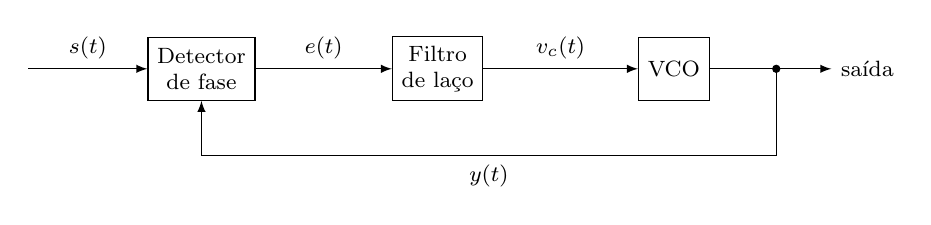
\begin{tikzpicture}[>=latex, font=\footnotesize]
\node[draw, rectangle, minimum height=0.8cm, align=center] (pd) at (0,0) {Detector\\ de fase};
\node[draw, rectangle, minimum height=0.8cm, align=center] (lpf) at (3,0) {Filtro\\ de laço};
\node[draw, rectangle, minimum height=0.8cm, align=center] (vco) at (6,0) {VCO};
\draw[->] (-2.2,0) -- node[above] {$s(t)$} (pd.west);
\draw[->] (pd.east) -- node[above] {$e(t)$} (lpf.west);
\draw[->] (lpf.east) -- node[above] {$v_c(t)$} (vco.west);
\draw[->] (vco.east) -- (8,0) node[right] {saída};
\draw[->] (7.3,0) -- (7.3,-1.1) -- node[below] {$y(t)$} (0,-1.1) -- (pd.south);
\fill (7.3,0) circle (1.5pt);
\end{tikzpicture}
\end{center}

\textbf{Componentes:}
\begin{itemize}
\item \textbf{Detector de fase (PD):} Compara fases de entrada e VCO
\item \textbf{Filtro de loop:} Passa-baixas, define dinâmica
\item \textbf{VCO:} Frequência controlada por tensão
\end{itemize}

\end{frame}

% ============================================

\begin{frame}{PLL: sinais de entrada e VCO}

\textbf{Entrada FM} (forma usada em análise PLL, equivalente a $\cos$ com 90° de defasagem):
\[
r(t) = A_c \sin[2\pi f_c t + \phi(t)], \quad \phi(t) = 2\pi k_f\!\int m(\tau)\,d\tau.
\]

\pause
\textbf{Saída do VCO} (em quadratura com a entrada para que o detector entregue $\sin$ do erro):
\[
y_v(t) = A_v \cos[2\pi f_c t + \phi_v(t)],
\]
\[
\boxed{\;\phi_v(t) = 2\pi k_v \int_0^t v(\tau)\,d\tau\;} \qquad (\text{Proakis 4.3.17})
\]
onde $k_v$ é a sensibilidade do VCO em Hz/V e $v(t)$ é a tensão de controle.

\pause
\textbf{Comparador de fase:} multiplicador analógico seguido de filtro passa-baixa que rejeita o termo em $2 f_c$.

\end{frame}

% ============================================

\begin{frame}{Detector de fase: derivação}

\textbf{Produto} $r(t)\,y_v(t)$ com $\omega_c \equiv 2\pi f_c$:
\[
A_c A_v \sin[\omega_c t + \phi]\,\cos[\omega_c t + \phi_v]
\]

\pause
\textbf{Identidade:} $\sin A\,\cos B = \tfrac{1}{2}[\sin(A+B) + \sin(A-B)]$. Com $A = \omega_c t + \phi$, $B = \omega_c t + \phi_v$:
\[
r\,y_v = \tfrac{A_c A_v}{2}\Bigl\{\underbrace{\sin[2\omega_c t + \phi + \phi_v]}_{2f_c\;\to\;\text{LPF rejeita}} + \sin[\phi - \phi_v]\Bigr\}
\]

\pause
\textbf{Após o LPF do comparador:}
\[
\boxed{\;e(t) = \tfrac{1}{2}A_v A_c\,\sin[\phi(t) - \phi_v(t)]\;} \qquad (\text{Proakis 4.3.18})
\]

\pause
\textbf{Observação:} o seno aparece naturalmente da identidade $\sin\!\cdot\!\cos$. Garante $e = 0$ exatamente em $\phi = \phi_v$ -- condição de \emph{lock}.

\end{frame}

% ============================================

\begin{frame}{Linearização e modelo do PLL}

\textbf{Erro de fase:} $\phi_e(t) \equiv \phi(t) - \phi_v(t)$.

\pause
\textbf{Hipótese de PLL travado} ($|\phi_e| \ll 1$): pela expansão $\sin x \approx x$,
\[
\sin[\phi(t) - \phi_v(t)] \approx \phi(t) - \phi_v(t) = \phi_e(t) \qquad (\text{Proakis 4.3.19})
\]
e o detector vira linear: $e(t) \approx \tfrac{1}{2}A_v A_c\,\phi_e(t)$.

\pause
\textbf{Modelo linearizado do PLL} (Proakis Fig 4.15):

\begin{center}
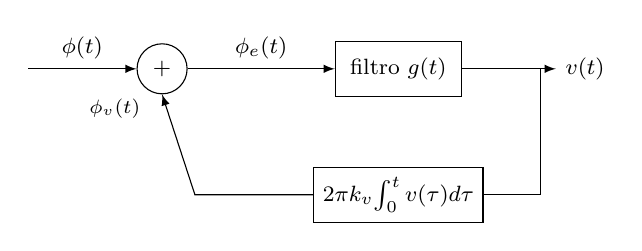
\begin{tikzpicture}[>=latex, every node/.style={font=\footnotesize}]
\node[draw, circle, minimum size=0.6cm] (sum) at (0,0) {$+$};
\node[draw, rectangle, minimum width=1.6cm, minimum height=0.7cm] (lf) at (3,0) {filtro $g(t)$};
\node[draw, rectangle, minimum width=2cm, minimum height=0.7cm] (vco) at (3,-1.6) {$2\pi k_v\!\int_0^t v(\tau)d\tau$};

\draw[->] (-1.7,0) -- node[above] {$\phi(t)$} (sum);
\draw[->] (sum) -- node[above] {$\phi_e(t)$} (lf);
\draw[->] (lf) -- ++(2,0) node[right] {$v(t)$};
\draw (lf.east) -- ++(1,0) -- ++(0,-1.6) -- (vco.east);
\draw[->] (vco.west) -- ++(-1.5,0) -- (sum.south);
\node[font=\scriptsize] at (-0.6,-0.5) {$\phi_v(t)$};
\end{tikzpicture}
\end{center}

\end{frame}

% ============================================

\begin{frame}{Equação do erro de fase}

Substituindo $\phi_v(t) = 2\pi k_v \!\int_0^t v(\tau)d\tau$ em $\phi_e = \phi - \phi_v$:
\[
\phi_e(t) = \phi(t) - 2\pi k_v \int_0^t v(\tau)\,d\tau \qquad (\text{Proakis 4.3.20})
\]

\pause
\textbf{Diferenciando:}
\[
\frac{d\phi_e(t)}{dt} + 2\pi k_v\,v(t) = \frac{d\phi(t)}{dt} \qquad (\text{4.3.21})
\]

\pause
\textbf{Filtro de loop:} $v(t) = \int_0^\infty \phi_e(\tau)\,g(t-\tau)\,d\tau$ -- convolução com $g(t)$.

\pause
\textbf{Substituindo:}
\[
\frac{d\phi_e}{dt} + 2\pi k_v\!\int_0^\infty\!\phi_e(\tau)\,g(t-\tau)\,d\tau = \frac{d\phi}{dt} \qquad (\text{4.3.22})
\]

\end{frame}

% ============================================

\begin{frame}{PLL no domínio da frequência}

\textbf{Transformada de Fourier} da equação integro-diferencial 4.3.22:
\[
(j2\pi f)\,\Phi_e(f) + 2\pi k_v\,\Phi_e(f)\,G(f) = (j2\pi f)\,\Phi(f) \qquad (\text{4.3.23})
\]

\pause
\textbf{Resolvendo para $\Phi_e(f)$:}
\[
\boxed{\;\Phi_e(f) = \frac{1}{1 + \dfrac{k_v}{jf}\,G(f)}\,\Phi(f)\;} \qquad (\text{4.3.24})
\]

\pause
\textbf{Tensão de controle $V(f) = \Phi_e(f)\,G(f)$:}
\[
V(f) = \frac{G(f)}{1 + \dfrac{k_v}{jf}\,G(f)}\,\Phi(f) \qquad (\text{4.3.25})
\]

\end{frame}

% ============================================

\begin{frame}{Demodulação FM via PLL}

\small\compacto

\textbf{Critério de projeto} (Proakis 4.3.26): para $|f| < W$ (banda da mensagem),
\[
\left|\dfrac{k_v\,G(f)}{jf}\right| \gg 1.
\]

\pause
Nessa faixa o denominador de 4.3.25 fica $\approx (k_v/jf)\,G(f)$:
\[
V(f) \approx \dfrac{j2\pi f}{2\pi k_v}\,\Phi(f) \qquad (\text{4.3.27})
\]

\pause
\textbf{No tempo:} $v(t) = \dfrac{1}{2\pi k_v}\,\dfrac{d\phi}{dt}$. Como $\dot\phi = 2\pi k_f\,m(t)$:
\[
\boxed{\;v(t) = \dfrac{k_f}{k_v}\,m(t)\;} \qquad (\text{4.3.28})
\]

A tensão de controle do VCO é proporcional à mensagem.

\end{frame}

% ============================================

\begin{frame}{Filtro de laço $G(s)$ e malha fechada $H(s)$}

\textbf{$G(s)$} é o \emph{filtro de loop} -- mesma função da derivação Proakis, com $s = j2\pi f$. É o que você \textbf{escolhe} no projeto.

\pause
\vspace{0.3cm}
\textbf{$H(s) = \Phi_v(s)/\Phi(s)$} é a \emph{função de transferência em malha fechada}, calculada a partir de $G$ e do ganho do VCO:
\[
\boxed{\;H(s) = \frac{2\pi k_v\,G(s)}{s + 2\pi k_v\,G(s)}\;}
\]

\pause
\vspace{0.3cm}
$H$ é o que \textbf{resulta} -- a relação entre o sinal de entrada e o sinal travado pelo VCO. Determina a dinâmica do laço (rapidez, amortecimento, banda).

\vspace{0.3cm}
Próximos slides: dois casos comuns de $G$ e o $H$ correspondente.

\end{frame}

% ============================================

\begin{frame}{Caso 1: filtro proporcional $G(s) = 1$}

\textbf{Escolha mais simples:} $G(s) = 1$ (sem dinâmica adicional, só ganho unitário).

\pause
\textbf{Substituindo na fórmula de $H$:}
\[
H(s) = \frac{2\pi k_v}{s + 2\pi k_v}
\]

\textbf{Sistema de 1ª ordem.} Polo único em $s = -2\pi k_v$, constante de tempo $\tau = 1/(2\pi k_v)$.

\pause
\vspace{0.3cm}
\textbf{Exemplo numérico} ($k_v = 50$\,kHz/V):
\[
2\pi k_v = 2\pi\cdot 50\,\text{kHz} = 3{,}14\!\times\!10^5\,\text{rad/s}
\]
\[
\tau = \frac{1}{3{,}14\!\times\!10^5} = 3{,}2\,\mu\text{s}, \qquad B_L = \frac{2\pi k_v}{4} = 78{,}5\,\text{kHz}
\]

\pause
\textbf{Limitação:} 1ª ordem não permite ajustar amortecimento independentemente. Aumentar $k_v$ acelera resposta mas degrada margem de estabilidade.

\end{frame}

% ============================================

\begin{frame}{Caso 2: filtro lag-lead}

\textbf{Topologia mais usada em receptores reais:} permite ajustar $\zeta$ e $\omega_n$ separadamente.

\pause
\vspace{0.2cm}
Substituindo na fórmula de $H$, obtém-se sistema de 2ª ordem padrão:
\[
\omega_n = \sqrt{\dfrac{2\pi k_v}{\tau_1}}, \qquad
\zeta = \dfrac{\omega_n}{2}\!\left(\tau_2 + \dfrac{1}{2\pi k_v}\right)
\]

\pause
\vspace{0.3cm}
\textbf{Projeto:} dado $\zeta$ e $f_n$ desejados, resolve-se para $\tau_1$ e $\tau_2$.

\pause
\vspace{0.2cm}
\textbf{Exemplo} ($k_v = 50$\,kHz/V, alvo $\zeta = 0{,}7$, $f_n = 30$\,kHz):
\[
\omega_n = 2\pi\cdot 30\,\text{kHz} = 1{,}88\!\times\!10^5\,\text{rad/s}
\]
\[
\tau_1 = \frac{2\pi k_v}{\omega_n^2} \approx 88\,\mu\text{s}, \qquad
\tau_2 = \frac{2\zeta}{\omega_n} - \frac{1}{2\pi k_v} \approx 7{,}3\,\mu\text{s}.
\]

\end{frame}

% ============================================

\begin{frame}{Visualização: Análise do PLL}

\begin{center}
\includegraphics[height=0.64\textheight,keepaspectratio]{figures/cap4/pll_analysis.pdf}
\end{center}

\end{frame}

% ============================================

\begin{frame}{Travamento do PLL}

\begin{center}
\includegraphics[height=0.6\textheight,keepaspectratio]{figures/cap4/pll_locking.pdf}
\end{center}

\small O VCO converge para a frequência de entrada. Após o travamento, $v_c(t) \propto m(t)$.

\end{frame}

% ============================================

\begin{frame}{Parâmetros do PLL: capture e lock}

\small\compacto

\textbf{Lock range} -- faixa onde o PLL \emph{mantém} o travamento já adquirido. Vale para qualquer ordem:
\[
\Delta f_{lock} \approx \frac{K_d K_v}{2\pi} \quad\text{(com $K_v$ em rad/s/V)}
\]

\pause
\textbf{Capture range} -- faixa onde o PLL \emph{adquire} o travamento partindo do destravado. Aqui a ordem importa:
\begin{itemize}\itemsep0pt
\item \textbf{1ª ordem} ($G=1$): não há transitório de aquisição -- $\Delta f_{capture} = \Delta f_{lock}$.
\item \textbf{2ª ordem} (lag-lead): há \emph{pull-in} com dinâmica de $\zeta, \omega_n$, e
\[
\Delta f_{capture} \approx 2\zeta f_n < \Delta f_{lock}
\]
\end{itemize}

\pause
\textbf{Exemplo} ($K_d = 1$\,V/rad, $k_v = 50$\,kHz/V): $\;\Delta f_{lock} = 50$\,kHz.

Com lag-lead de $\zeta = 0{,}7$, $f_n = 30$\,kHz: $\Delta f_{capture} = 42$\,kHz $< 50$\,kHz.

\pause
\textbf{Para FM broadcast} ($\Delta f = 75$\,kHz): aumentar $k_v$ para $\sim$100\,kHz/V garante $\Delta f_{lock} > 75$\,kHz.

\end{frame}

% ============================================

\begin{frame}{Convenção dos ganhos do PLL}

As três fórmulas de parâmetros ($\Delta f_{lock}$, $\Delta f_{capture}$, $B_L$) usam a mesma combinação $K_d K_v$. Antes dos exemplos numéricos, fixar unidades:

\pause
\vspace{0.3cm}
\begin{itemize}\itemsep0.3em
\item \textbf{$K_d$} -- ganho do detector de fase, em \textbf{V/rad}.

Vem da derivação: $K_d = \frac{1}{2}A_c A_v$.

\pause
\item \textbf{$K_v$} -- ganho do VCO, em \textbf{rad/s/V}.

Relação com $k_v$ em Hz/V: $\;K_v = 2\pi k_v$.

\pause
\item \textbf{$K_d K_v$} -- \emph{ganho de loop em malha aberta}, em \textbf{rad/s}.

Aparece em todas as fórmulas dinâmicas (lock range, banda, polos).
\end{itemize}

\end{frame}

% ============================================

\begin{frame}{Largura de banda do loop $B_L$}

\textbf{$B_L$} determina resposta dinâmica e rejeição de ruído do PLL.

\vspace{0.3cm}
\textbf{Para 1ª ordem} (filtro proporcional):
\[
\boxed{\;B_L = \frac{K_d K_v}{4}\;}
\]

\pause
\vspace{0.3cm}
\textbf{Exemplo numérico} ($K_d = 1$\,V/rad, $k_v = 50$\,kHz/V):
\[
K_d K_v = 1 \cdot 2\pi \cdot 50\,\text{kHz} = 3{,}14\!\times\!10^5\,\text{rad/s}
\]
\[
B_L = \frac{3{,}14\!\times\!10^5}{4} = 78{,}5\,\text{kHz}
\]

\end{frame}

% ============================================

\begin{frame}{Trade-off de banda do loop}

\textbf{$B_L$ largo:}
\begin{itemize}\itemsep0pt
\item Resposta rápida -- PLL acompanha variações rápidas de fase.
\item \textbf{Mais ruído} passa pela saída.
\end{itemize}

\pause
\vspace{0.3cm}
\textbf{$B_L$ estreito:}
\begin{itemize}\itemsep0pt
\item Saída mais limpa (ruído rejeitado).
\item PLL \textbf{lento} -- pode não acompanhar variações rápidas da mensagem.
\end{itemize}

\pause
\vspace{0.3cm}
\textbf{Critério prático:} $B_L \gtrsim f_{m,\max}$ da mensagem para garantir tracking.

\textbf{Exemplo:} áudio FM tem $f_{m,\max} = 15$\,kHz. O $B_L = 78{,}5$\,kHz do exemplo anterior acompanha confortavelmente, com margem para o ruído.

\end{frame}

% ============================================

\begin{frame}{Aplicações do PLL}

\small
O PLL é versátil e amplamente usado:

\begin{columns}[T]
\column{0.5\textwidth}
\begin{enumerate}
\item Demodulação FM: receptores de rádio e TV, com boa linearidade e rejeição de amplitude.
\item Síntese de frequência: múltiplos de uma referência, em geradores de RF.
\item Recuperação de portadora: demodulação coerente em sistemas digitais.
\end{enumerate}
\column{0.5\textwidth}
\begin{enumerate}\setcounter{enumi}{3}
\item Recuperação de clock: sincronização de dados e interfaces seriais.
\item Controle de motor: velocidade precisa.
\end{enumerate}
\end{columns}

\end{frame}

% ============================================

\section{Geração de FM}

\begin{frame}{Geração Direta de FM}

\textbf{Modulador direto com VCO:}

\begin{center}
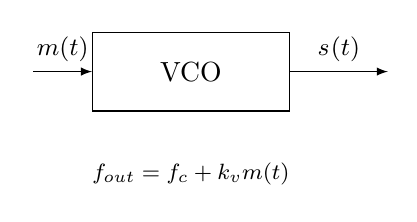
\begin{tikzpicture}[>=latex]
\node[draw, rectangle, minimum width=2.5cm, minimum height=1cm] (vco) at (0,0) {VCO};
\draw[->] (-2,0) -- node[above, font=\small] {$m(t)$} (vco.west);
\draw[->] (vco.east) -- node[above, font=\small] {$s_{\FM}(t)$} (2.5,0);
\node[below of=vco, node distance=1.3cm, font=\footnotesize] {$f_{out} = f_c + k_v m(t)$};
\end{tikzpicture}
\end{center}

\textbf{Características:} simples e direto. VCO implementado com varactor, capacitor variável, ou similares.

\pause
\vspace{0.2cm}
\textbf{Problema:} instabilidade de frequência. $f_c$ deriva com temperatura, componentes e tensão de alimentação. É difícil obter $f_c$ precisa e estável.

\pause
\textbf{Solução:} usar método indireto de Armstrong.

\end{frame}

% ============================================

\begin{frame}{Método de Armstrong: ideia geral}

\textbf{Ideia central:} gerar NBFM estável a partir de cristal e depois multiplicar a frequência até obter WBFM.

\vspace{0.4cm}
\pause
\textbf{Processo:}

\begin{enumerate}
\item Gerar NBFM com $\beta$ pequeno e $f_c$ estável de cristal.
\item Multiplicar frequência por $n$, o que multiplica também $f_c$, $\Delta f$ e $\beta$ pelo mesmo fator.
\item Converter para a banda desejada via mixer.
\item Repetir multiplicação se necessário.
\end{enumerate}

\pause
\vspace{0.3cm}
\textbf{Efeito da multiplicação por $n$:}
\[
f_c \to n f_c, \qquad \beta \to n\beta, \qquad \Delta f \to n\Delta f.
\]

\end{frame}

% ============================================

\begin{frame}{Modulador NBFM: núcleo do Armstrong}

\textbf{Sintetizar} $s_{\NBFM}(t) = A_c\cos(2\pi f_1 t) - A_c\,\phi(t)\sin(2\pi f_1 t)$ \textbf{com} $\phi(t) = 2\pi k_f\!\int m(\tau)d\tau$:

\begin{center}
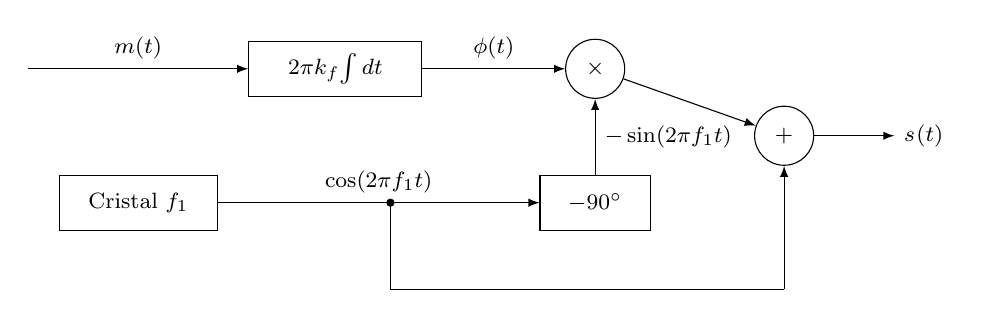
\begin{tikzpicture}[>=latex, every node/.style={font=\footnotesize}]
\node[draw, rectangle, minimum width=2.2cm, minimum height=0.7cm] (int) at (2.5,1.7) {$2\pi k_f\!\int dt$};
\node[draw, circle, minimum size=0.75cm] (mul) at (5.8,1.7) {$\times$};
\node[draw, circle, minimum size=0.75cm] (sum) at (8.2,0.85) {$+$};
\node[draw, rectangle, minimum width=2cm, minimum height=0.7cm] (osc) at (0,0) {Cristal $f_1$};
\node[draw, rectangle, minimum width=1.4cm, minimum height=0.7cm] (sh) at (5.8,0) {$-90^\circ$};

\draw[->] (-1.4,1.7) -- node[above] {$m(t)$} (int);
\draw[->] (int) -- node[above] {$\phi(t)$} (mul);
\draw[->] (mul) -- (sum);
\draw[->] (osc) -- node[above] {$\cos(2\pi f_1 t)$} (sh);
\draw[->] (sh) -- node[right] {$-\sin(2\pi f_1 t)$} (mul);
\fill (3.2,0) circle (1.5pt);
\draw (3.2,0) -- (3.2,-1.1) -- (8.2,-1.1);
\draw[->] (8.2,-1.1) -- (sum);
\draw[->] (sum) -- ++(1.4,0) node[right] {$s_{\NBFM}(t)$};
\end{tikzpicture}
\end{center}

\textbf{Cristal} fornece $f_1$ estável; \textbf{integrador} converte $m(t)$ em $\phi(t)$; \textbf{defasador, multiplicador e somador} montam a soma em quadratura. Como $f_1$ não passa pelo modulador, sua estabilidade é preservada.

\end{frame}

% ============================================

\begin{frame}{Cadeia Armstrong completa}

\begin{center}
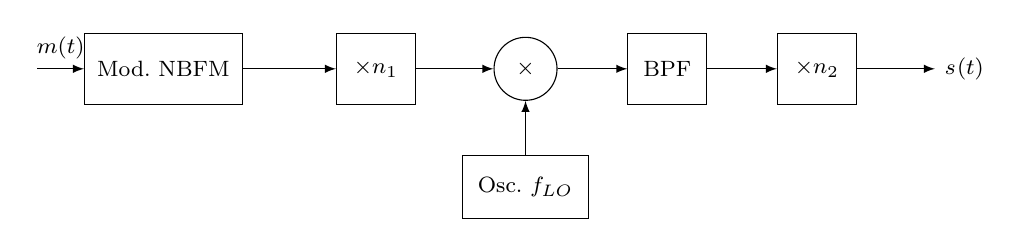
\begin{tikzpicture}[>=latex, every node/.style={font=\footnotesize}]
\node[draw, rectangle, minimum width=2cm, minimum height=0.9cm] (nbfm) at (0,0) {Mod.\ NBFM};
\node[draw, rectangle, minimum width=1cm, minimum height=0.9cm] (n1) at (2.7,0) {$\times n_1$};
\node[draw, circle, minimum size=0.8cm] (mix) at (4.6,0) {$\times$};
\node[draw, rectangle, minimum width=1cm, minimum height=0.9cm] (bpf) at (6.4,0) {BPF};
\node[draw, rectangle, minimum width=1cm, minimum height=0.9cm] (n2) at (8.3,0) {$\times n_2$};
\node[draw, rectangle, minimum width=1.6cm, minimum height=0.8cm] (lo) at (4.6,-1.5) {Osc.\ $f_{LO}$};

\draw[->] (-1.6,0) -- node[above] {$m(t)$} (nbfm);
\draw[->] (nbfm) -- (n1);
\draw[->] (n1) -- (mix);
\draw[->] (mix) -- (bpf);
\draw[->] (bpf) -- (n2);
\draw[->] (n2) -- ++(1.5,0) node[right] {$s_{\FM}(t)$};
\draw[->] (lo) -- (mix);
\end{tikzpicture}
\end{center}

\textbf{Em cada estágio:}
\begin{itemize}\itemsep0pt
\item Saída do NBFM: $f_1, \Delta f_1$ com $\beta_1 \ll 1$.
\item Após $\times n_1$: $n_1 f_1,\, n_1 \Delta f_1,\, n_1\beta_1$.
\item Mixer produz $f_2 \pm f_{LO}$; BPF seleciona uma das duas; $\Delta f$ inalterado.
\item Após $\times n_2$: $n_2 f_3,\, n_1 n_2 \Delta f_1$.
\end{itemize}

\textbf{Liberdade de projeto:} produto $n_1 n_2$ ajusta $\Delta f_{\text{final}}$; $f_{LO}$ ajusta $f_c$ independentemente.

\end{frame}

% ============================================

\begin{frame}{Cenário A: especificação}

\textbf{Meta:} $f_c = 100$\,MHz, $\Delta f = 75$\,kHz, $f_{m,\max} = 15$\,kHz.

\pause
\textbf{Estágio NBFM} (cristal de 200\,kHz, $\Delta f_1$ pequeno):
\[
f_1 = 200\,\text{kHz}, \quad \Delta f_1 = 25\,\text{Hz} \;\Rightarrow\; \beta_1 \approx 1{,}7\!\times\!10^{-3}.
\]

\pause
\textbf{Banda Carson após NBFM:}
\[
B_0 = 2(\Delta f_1 + f_{m,\max}) = 2(0{,}025 + 15)\,\text{kHz} \approx 30\,\text{kHz}.
\]

\pause
\textbf{Multiplicação total:} $N = \dfrac{75\,000}{25} = 3000 = n_1\cdot n_2 = 60\cdot 50$.

\end{frame}

% ============================================

\begin{frame}{Cenário A: após $\times n_1 = 60$}

Não-linearidade do multiplicador gera comb $k f_1$, $k \in \{1, 2, 3, \ldots\}$. Filtro LC sintonizado em $60 f_1 = 12$\,MHz seleciona o 60º harmônico.

\begin{center}
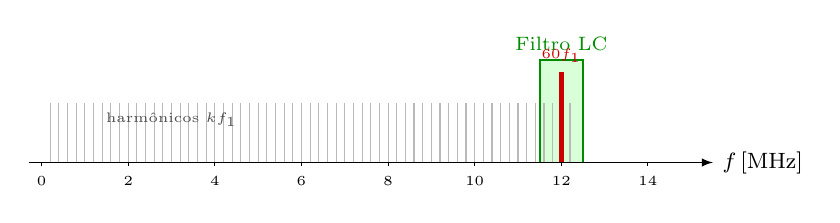
\begin{tikzpicture}[>=latex, x=0.55cm, y=0.5cm, every node/.style={font=\footnotesize}]
\draw[->] (-0.3,0) -- (15.5,0) node[right] {$f$\,[MHz]};
\fill[green!15] (11.5,0) rectangle (12.5,2.6);
\draw[thick, green!55!black] (11.5,0) -- (11.5,2.6) -- (12.5,2.6) -- (12.5,0);
\node[green!55!black, anchor=south, font=\scriptsize] at (12,2.6) {Filtro LC};
\foreach \k in {1,...,59,61,...,70} {
  \pgfmathsetmacro{\xpos}{\k * 0.2}
  \draw[gray!55, thin] (\xpos,0) -- (\xpos,1.5);
}
\draw[ultra thick, red!80!black] (12,0) -- (12,2.3);
\node[red!80!black, anchor=south, font=\tiny] at (12,2.3) {$60 f_1$};
\node[font=\tiny, gray!60!black, anchor=north] at (3,1.5) {harmônicos $k f_1$};
\foreach \x in {0,2,4,6,8,10,12,14} {
  \draw (\x,0) -- (\x,-0.1);
  \node[anchor=north, font=\tiny] at (\x,-0.1) {\x};
}
\end{tikzpicture}
\end{center}

\textbf{Saída:} $f_2 = 12$\,MHz, $\Delta f_2 = 60\cdot 25 = 1{,}5$\,kHz.\quad
\textbf{Banda:} $B_1 = 2(1{,}5 + 15) = 33$\,kHz (ainda dominada por $f_m$).

\end{frame}

% ============================================

\begin{frame}{Cenário A: saída do mixer}

\textbf{Necessidade:} $f_3 = 100/50 = 2$\,MHz.\quad
\textbf{Escolha:} $f_{LO} = 10$\,MHz (subtrativo).

\begin{center}
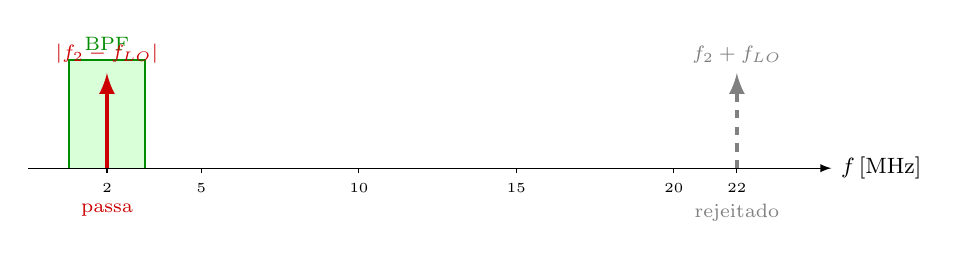
\begin{tikzpicture}[>=latex, x=0.4cm, y=0.55cm, every node/.style={font=\footnotesize}]
\draw[->] (-0.5,0) -- (25,0) node[right] {$f$\,[MHz]};
\fill[green!15] (0.8,0) rectangle (3.2,2.5);
\draw[thick, green!55!black] (0.8,0) -- (0.8,2.5) -- (3.2,2.5) -- (3.2,0);
\node[green!55!black, anchor=south, font=\scriptsize] at (2,2.5) {BPF};
\draw[ultra thick, red!80!black, ->] (2,0) -- (2,2.2);
\node[red!80!black, anchor=south, font=\scriptsize] at (2,2.2) {$|f_2-f_{LO}|$};
\node[red!80!black, anchor=north, font=\scriptsize] at (2,-0.6) {passa};
\draw[ultra thick, gray, dashed, ->] (22,0) -- (22,2.2);
\node[gray, anchor=south, font=\scriptsize] at (22,2.2) {$f_2+f_{LO}$};
\node[gray, anchor=north, font=\scriptsize] at (22,-0.6) {rejeitado};
\foreach \x in {2,5,10,15,20,22} {
  \draw (\x,0) -- (\x,-0.12);
  \node[anchor=north, font=\tiny] at (\x,-0.12) {\x};
}
\end{tikzpicture}
\end{center}

\textbf{BPF em 2\,MHz} entrega $f_3 = 2$\,MHz, $\Delta f_3 = 1{,}5$\,kHz.\quad
\textbf{Banda:} $B_2 = 33$\,kHz (mixer não muda $\Delta f$ nem $f_m$).

\end{frame}

% ============================================

\begin{frame}{Cenário A: após $\times n_2 = 50$}

Comb $k f_3$ para $k \in \{1, 2, 3, \ldots\}$. Filtro LC em $50 f_3 = 100$\,MHz seleciona o 50º harmônico.

\begin{center}
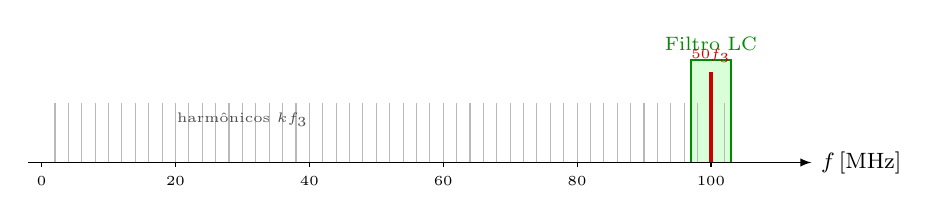
\begin{tikzpicture}[>=latex, x=0.085cm, y=0.5cm, every node/.style={font=\footnotesize}]
\draw[->] (-2,0) -- (115,0) node[right] {$f$\,[MHz]};
\fill[green!15] (97,0) rectangle (103,2.6);
\draw[thick, green!55!black] (97,0) -- (97,2.6) -- (103,2.6) -- (103,0);
\node[green!55!black, anchor=south, font=\scriptsize] at (100,2.6) {Filtro LC};
\foreach \k in {1,...,49,51,...,55} {
  \pgfmathsetmacro{\xpos}{\k * 2}
  \draw[gray!55, thin] (\xpos,0) -- (\xpos,1.5);
}
\draw[ultra thick, red!80!black] (100,0) -- (100,2.3);
\node[red!80!black, anchor=south, font=\tiny] at (100,2.3) {$50 f_3$};
\node[font=\tiny, gray!60!black, anchor=north] at (30,1.5) {harmônicos $k f_3$};
\foreach \x in {0,20,40,60,80,100} {
  \draw (\x,0) -- (\x,-0.12);
  \node[anchor=north, font=\tiny] at (\x,-0.12) {\x};
}
\end{tikzpicture}
\end{center}

\textbf{Saída final:} $f_c = 100$\,MHz \checkmark,\;\; $\Delta f = 75$\,kHz \checkmark,\;\; $\beta = 5$ (WBFM).

\textbf{Banda:} $B_3 = 2(75 + 15) = 180$\,kHz -- agora dominada por $\Delta f$.

\end{frame}

% ============================================

\begin{frame}{Cenário B: especificação}

\textbf{Meta:} $f_c = 100$\,MHz, $\Delta f = 5$\,kHz, $f_{m,\max} = 3$\,kHz (rádio comercial de voz).

\pause
\textbf{Estágio NBFM} (mesmo cristal de 200\,kHz):
\[
f_1 = 200\,\text{kHz}, \quad \Delta f_1 = 25\,\text{Hz} \;\Rightarrow\; \beta_1 \approx 8{,}3\!\times\!10^{-3}.
\]

\pause
\textbf{Banda Carson após NBFM:} $B_0 = 2(0{,}025 + 3)\,\text{kHz} \approx 6\,\text{kHz}$.

\pause
\textbf{Multiplicação total} usando \emph{multiplicadores físicos} ($\times 2$ dobradores e $\times 5$ quintuplicadores):
\[
N = \frac{5000}{25} = 200 = n_1\cdot n_2 = \underbrace{8}_{\times 2\cdot\times 2\cdot\times 2}\cdot\underbrace{25}_{\times 5\cdot\times 5}.
\]

\textbf{Cadeia completa:} 3 dobradores $\to$ mixer $\to$ 2 quintuplicadores.

\end{frame}

% ============================================

\begin{frame}{Cenário B: após $\times n_1 = 8$}

Cadeia $\times 2 \cdot \times 2 \cdot \times 2$: cada estágio Classe C gera comb $k f_{\text{in}}$ e o filtro LC seleciona o 2º harmônico. Resultado equivalente a um $\times 8$.

\begin{center}
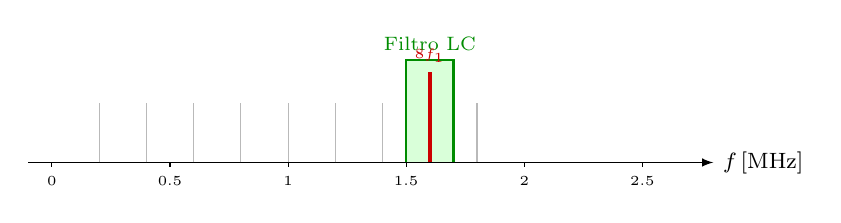
\begin{tikzpicture}[>=latex, x=3.0cm, y=0.5cm, every node/.style={font=\footnotesize}]
\draw[->] (-0.1,0) -- (2.8,0) node[right] {$f$\,[MHz]};
\fill[green!15] (1.5,0) rectangle (1.7,2.6);
\draw[thick, green!55!black] (1.5,0) -- (1.5,2.6) -- (1.7,2.6) -- (1.7,0);
\node[green!55!black, anchor=south, font=\scriptsize] at (1.6,2.6) {Filtro LC};
\foreach \k in {1,...,7,9,...,12} {
  \pgfmathsetmacro{\xpos}{\k * 0.2}
  \draw[gray!55, thin] (\xpos,0) -- (\xpos,1.5);
}
\draw[ultra thick, red!80!black] (1.6,0) -- (1.6,2.3);
\node[red!80!black, anchor=south, font=\tiny] at (1.6,2.3) {$8 f_1$};
\foreach \x in {0,0.5,1,1.5,2,2.5} {
  \draw (\x,0) -- (\x,-0.12);
  \node[anchor=north, font=\tiny] at (\x,-0.12) {\x};
}
\end{tikzpicture}
\end{center}

\textbf{Saída:} $f_2 = 8 \cdot 200\,\text{kHz} = 1{,}6$\,MHz,\;\; $\Delta f_2 = 8 \cdot 25\,\text{Hz} = 200$\,Hz.

\textbf{Banda:} $B_1 = 2(0{,}2 + 3) = 6{,}4$\,kHz.

\end{frame}

% ============================================

\begin{frame}{Cenário B: saída do mixer}

\textbf{Necessidade:} $f_3 = 100/25 = 4$\,MHz.\quad
Como $f_3 > f_2 = 1{,}6$\,MHz, escolhemos $f_{LO} = 2{,}4$\,MHz (\textbf{aditivo}).

\begin{center}
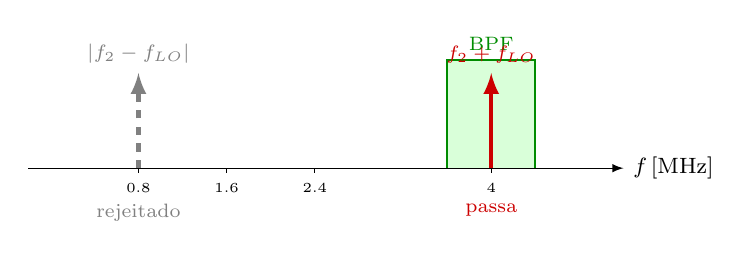
\begin{tikzpicture}[>=latex, x=1.4cm, y=0.55cm, every node/.style={font=\footnotesize}]
\draw[->] (-0.2,0) -- (5.2,0) node[right] {$f$\,[MHz]};
\fill[green!15] (3.6,0) rectangle (4.4,2.5);
\draw[thick, green!55!black] (3.6,0) -- (3.6,2.5) -- (4.4,2.5) -- (4.4,0);
\node[green!55!black, anchor=south, font=\scriptsize] at (4,2.5) {BPF};
\draw[ultra thick, gray, dashed, ->] (0.8,0) -- (0.8,2.2);
\node[gray, anchor=south, font=\scriptsize] at (0.8,2.2) {$|f_2-f_{LO}|$};
\node[gray, anchor=north, font=\scriptsize] at (0.8,-0.6) {rejeitado};
\draw[ultra thick, red!80!black, ->] (4,0) -- (4,2.2);
\node[red!80!black, anchor=south, font=\scriptsize] at (4,2.2) {$f_2+f_{LO}$};
\node[red!80!black, anchor=north, font=\scriptsize] at (4,-0.6) {passa};
\foreach \x in {0.8,1.6,2.4,4} {
  \draw (\x,0) -- (\x,-0.12);
  \node[anchor=north, font=\tiny] at (\x,-0.12) {\x};
}
\end{tikzpicture}
\end{center}

\textbf{BPF em 4\,MHz} entrega $f_3 = 4$\,MHz, $\Delta f_3 = 200$\,Hz.\quad
\textbf{Banda:} $B_2 = 6{,}4$\,kHz.

\end{frame}

% ============================================

\begin{frame}{Cenário B: após $\times n_2 = 25$}

Cadeia $\times 5 \cdot \times 5$: cada estágio Classe C com filtro LC selecionando o 5º harmônico. Resultado equivalente a um $\times 25$.

\begin{center}
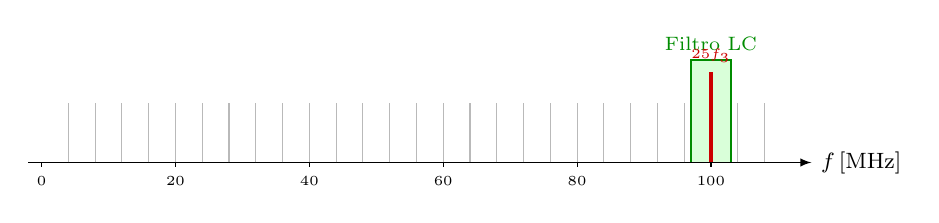
\begin{tikzpicture}[>=latex, x=0.085cm, y=0.5cm, every node/.style={font=\footnotesize}]
\draw[->] (-2,0) -- (115,0) node[right] {$f$\,[MHz]};
\fill[green!15] (97,0) rectangle (103,2.6);
\draw[thick, green!55!black] (97,0) -- (97,2.6) -- (103,2.6) -- (103,0);
\node[green!55!black, anchor=south, font=\scriptsize] at (100,2.6) {Filtro LC};
\foreach \k in {1,...,24,26,27} {
  \pgfmathsetmacro{\xpos}{\k * 4}
  \draw[gray!55, thin] (\xpos,0) -- (\xpos,1.5);
}
\draw[ultra thick, red!80!black] (100,0) -- (100,2.3);
\node[red!80!black, anchor=south, font=\tiny] at (100,2.3) {$25 f_3$};
\foreach \x in {0,20,40,60,80,100} {
  \draw (\x,0) -- (\x,-0.12);
  \node[anchor=north, font=\tiny] at (\x,-0.12) {\x};
}
\end{tikzpicture}
\end{center}

\textbf{Saída final:} $f_c = 25 \cdot 4 = 100$\,MHz \checkmark,\;\; $\Delta f = 25 \cdot 200 = 5$\,kHz \checkmark,\;\; $\beta \approx 1{,}67$.

\textbf{Banda:} $B_3 = 2(5 + 3) = 16$\,kHz.

\end{frame}

% ============================================

\begin{frame}[shrink=10]{Expansão de banda na cadeia Armstrong}

A multiplicação $\times n$ multiplica $\Delta f$ por $n$, mas \textbf{não} muda $f_m$. Logo, a banda Carson cresce conforme $\Delta f$ supera $f_m$.

\begin{center}
\footnotesize
\begin{tabular}{lcccc}
\toprule
Estágio & $f_c$ & $\Delta f$ & $\beta$ & $B = 2(\Delta f + f_m)$ \\
\midrule
\multicolumn{5}{l}{\emph{Cenário A} ($f_m = 15$\,kHz)} \\
NBFM             & 200\,kHz  & 25\,Hz     & 0{,}0017 & 30\,kHz  \\
$\times 60$      & 12\,MHz   & 1{,}5\,kHz & 0{,}1    & 33\,kHz  \\
mixer            & 2\,MHz    & 1{,}5\,kHz & 0{,}1    & 33\,kHz  \\
$\times 50$      & 100\,MHz  & 75\,kHz    & 5        & \textbf{180\,kHz} \\
\midrule
\multicolumn{5}{l}{\emph{Cenário B} ($f_m = 3$\,kHz)} \\
NBFM             & 200\,kHz   & 25\,Hz   & 0{,}0083 & 6\,kHz   \\
$\times 8$       & 1{,}6\,MHz & 200\,Hz  & 0{,}067  & 6{,}4\,kHz \\
mixer            & 4\,MHz     & 200\,Hz  & 0{,}067  & 6{,}4\,kHz \\
$\times 25$      & 100\,MHz   & 5\,kHz   & 1{,}67   & \textbf{16\,kHz}  \\
\bottomrule
\end{tabular}
\end{center}

\small
\textbf{Padrão:} enquanto $\beta \ll 1$ a banda quase não cresce ($\approx 2 f_m$). Só no estágio final, com $\beta \gtrsim 1$, a banda passa a ser dominada por $\Delta f$.

\end{frame}

% ============================================

\begin{frame}{Resumo dos dois cenários}

\begin{center}
\footnotesize
\begin{tabular}{lcc}
\toprule
Parâmetro & Cenário A (broadcast) & Cenário B (voz NBFM) \\
\midrule
$f_c$ final            & 100\,MHz       & 100\,MHz       \\
$\Delta f$ final       & 75\,kHz        & 5\,kHz         \\
$f_{m,\max}$           & 15\,kHz        & 3\,kHz         \\
$\beta$ final          & 5 (WBFM)       & 1{,}67         \\
\midrule
$f_1, \Delta f_1$      & 200\,kHz, 25\,Hz & 200\,kHz, 25\,Hz \\
$N = n_1 n_2$          & 3000 = 60$\cdot$50 & 200 = $2^3\cdot 5^2$ = 8$\cdot$25 \\
Cadeia                 & --                 & 3 dobr. + 2 quint. \\
$f_{LO}$               & 10\,MHz (subtr.)   & 2{,}4\,MHz (aditivo) \\
BPF passa              & 2\,MHz             & 4\,MHz         \\
BPF rejeita            & 22\,MHz            & 0{,}8\,MHz     \\
\bottomrule
\end{tabular}
\end{center}

\small
\textbf{Observação:} mesmo cristal e mesma $f_c$ final, mas $\Delta f$ muito diferentes. A flexibilidade vem da escolha de $N$ e do sentido do mixer.

\end{frame}

% ============================================

\section{Receptor Superheterodino}

\begin{frame}{Várias estações na mesma antena}

A antena recebe \textbf{toda} a faixa FM (88--108\,MHz), com canais espaçados de 200\,kHz. Para ouvir uma estação só, é preciso \emph{filtrar} apenas o canal desejado e rejeitar os adjacentes.

\begin{center}
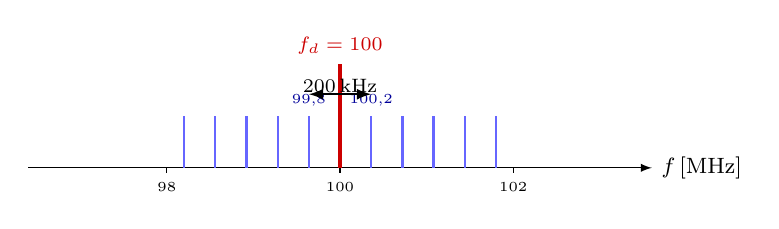
\begin{tikzpicture}[>=latex, x=2.2cm, y=0.55cm, every node/.style={font=\footnotesize}]
\draw[->] (-0.2,0) -- (3.4,0) node[right] {$f$\,[MHz]};
% Estações vizinhas (azul)
\foreach \k in {-5,-4,-3,-2,-1,1,2,3,4,5} {
  \pgfmathsetmacro{\xpos}{1.6 + \k * 0.18}
  \draw[blue!60, thick] (\xpos,0) -- (\xpos,1.2);
}
% Estação desejada em 100 MHz
\draw[ultra thick, red!80!black] (1.6,0) -- (1.6,2.4);
\node[red!80!black, anchor=south, font=\scriptsize] at (1.6,2.4) {$f_d = 100$};
% Vizinhas marcadas
\node[blue!60!black, font=\tiny, anchor=south] at (1.42,1.2) {99,8};
\node[blue!60!black, font=\tiny, anchor=south] at (1.78,1.2) {100,2};
% Espaçamento
\draw[<->, thick] (1.42,1.7) -- (1.78,1.7);
\node[font=\scriptsize] at (1.6,1.9) {200\,kHz};
% Ticks
\foreach \x/\lab in {0.6/{98},1.6/{100},2.6/{102}} {
  \draw (\x,0) -- (\x,-0.12);
  \node[anchor=north, font=\tiny] at (\x,-0.12) {\lab};
}
\end{tikzpicture}
\end{center}

\textbf{Objetivo do filtro RF:} passar 100\,MHz, atenuar 99,8 e 100,2\,MHz (vizinhas a apenas 200\,kHz).

\end{frame}

% ============================================

\begin{frame}[shrink=8]{Filtrar direto em $f_c$ é difícil}

\textbf{Seletividade exigida:} $Q = \dfrac{f_c}{B_{\text{canal}}} = \dfrac{100\,\text{MHz}}{200\,\text{kHz}} = 500$.

\pause
\textbf{Conflito $Q$ alto vs.\ sintonia.} Olhando as tecnologias de filtro:

\begin{center}
\footnotesize
\begin{tabular}{lccc}
\toprule
Tecnologia & $Q$ típico & Sintonizável? & Comentário \\
\midrule
LC paralelo (varactor) & 50--200 & \textbf{sim}  & $Q$ insuficiente \\
Cerâmico               & 200--1000 & não         & freq.\ fixa \\
Cristal de quartzo     & $10^3$--$10^5$ & não    & freq.\ fixa \\
SAW                    & 5000--20000 & não        & freq.\ fixa \\
\bottomrule
\end{tabular}
\end{center}

\pause
\textbf{Quem tem $Q \geq 500$ não é tunável.}\quad \textbf{Quem é tunável (LC) não atinge $Q = 500$.}

\pause
\textbf{Visualização:} mover o filtro pelo eixo $f$ enquanto mantém $B = 200$\,kHz:
\begin{center}
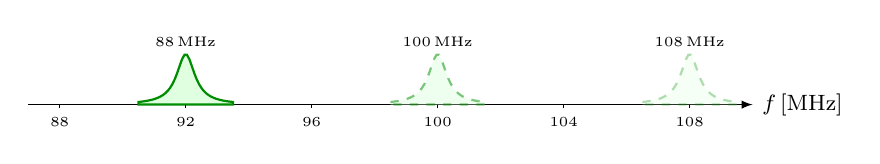
\begin{tikzpicture}[>=latex, x=0.4cm, y=0.4cm, every node/.style={font=\footnotesize}]
\draw[->] (-1,0) -- (22,0) node[right] {$f$\,[MHz]};
\draw[thick, green!55!black, fill=green!12] plot[domain=-1.5:1.5, samples=40] (4 + \x, {1.6/(1+(\x/0.35)^2)}) -- (5.5,0) -- (2.5,0) -- cycle;
\draw[thick, green!55!black, dashed, fill=green!12, opacity=0.5] plot[domain=-1.5:1.5, samples=40] (12 + \x, {1.6/(1+(\x/0.35)^2)}) -- (13.5,0) -- (10.5,0) -- cycle;
\draw[thick, green!55!black, dashed, fill=green!12, opacity=0.3] plot[domain=-1.5:1.5, samples=40] (20 + \x, {1.6/(1+(\x/0.35)^2)}) -- (21.5,0) -- (18.5,0) -- cycle;
\node[font=\tiny] at (4,2.0) {88\,MHz};
\node[font=\tiny] at (12,2.0) {100\,MHz};
\node[font=\tiny] at (20,2.0) {108\,MHz};
\foreach \x in {0,4,8,12,16,20} {
  \draw (\x,0) -- (\x,-0.1);
  \pgfmathtruncatemacro{\flab}{\x + 88}
  \node[anchor=north, font=\tiny] at (\x,-0.1) {\flab};
}
\end{tikzpicture}
\end{center}

\textbf{Conclusão:} filtro $Q=500$ e tunável de 88--108\,MHz é inviável.

\end{frame}

% ============================================

\begin{frame}{Solução: frequência intermediária fixa}

\textbf{Ideia:} em vez de mover o filtro, \textbf{mover o sinal} até uma frequência intermediária IF \emph{fixa}, onde um único filtro de alto $Q$ basta.

\begin{center}
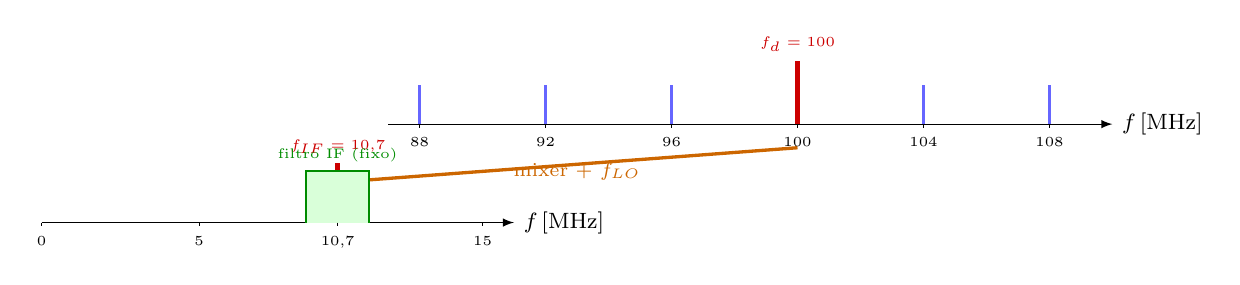
\begin{tikzpicture}[>=latex, x=0.4cm, y=0.5cm, every node/.style={font=\footnotesize}]
% Eixo
\draw[->] (-1,0) -- (22,0) node[right] {$f$\,[MHz]};
% Estações na faixa RF
\foreach \k in {0,4,8,12,16,20} {
  \draw[blue!60, thick] (\k,0) -- (\k,1.0);
}
\draw[ultra thick, red!80!black] (12,0) -- (12,1.6);
\node[red!80!black, anchor=south, font=\tiny] at (12,1.6) {$f_d = 100$};
% Seta do mixer
\draw[->, very thick, orange!80!black] (12,-0.6) -- (-3,-1.5);
\node[orange!80!black, font=\scriptsize] at (5,-1.2) {mixer + $f_{LO}$};
% IF axis (deslocada)
\draw[->] (-12,-2.5) -- (3,-2.5) node[right] {$f$\,[MHz]};
\draw[ultra thick, red!80!black] (-2.6,-2.5) -- (-2.6,-1.0);
\node[red!80!black, anchor=south, font=\tiny] at (-2.6,-1.0) {$f_{IF} = 10{,}7$};
% Filtro IF
\fill[green!15] (-3.6,-2.5) rectangle (-1.6,-1.2);
\draw[thick, green!55!black] (-3.6,-2.5) -- (-3.6,-1.2) -- (-1.6,-1.2) -- (-1.6,-2.5);
\node[green!55!black, anchor=south, font=\tiny] at (-2.6,-1.2) {filtro IF (fixo)};
% Ticks IF
\foreach \x/\lab in {-12/0,-7/5,-2.6/{10,7},2/15} {
  \draw (\x,-2.5) -- (\x,-2.6);
  \node[anchor=north, font=\tiny] at (\x,-2.6) {\lab};
}
% Ticks RF
\foreach \x in {0,4,8,12,16,20} {
  \draw (\x,0) -- (\x,-0.1);
  \pgfmathtruncatemacro{\flab}{\x + 88}
  \node[anchor=north, font=\tiny] at (\x,-0.1) {\flab};
}
\end{tikzpicture}
\end{center}

\textbf{Trocou-se um problema por outro:} agora o filtro é fixo (fácil), e o que sintoniza é o oscilador local $f_{LO}$ (também fácil -- VCO ajustável).

\end{frame}

% ============================================

\begin{frame}{Relação do superheterodino}

A mistura entre o sinal recebido e o oscilador local produz duas componentes; o filtro IF seleciona uma delas:
\[
\boxed{\;f_{IF} = |f_{RF} - f_{LO}|\;}
\]

\pause
\textbf{Para sintonizar $f_{RF}$:} basta ajustar $f_{LO}$ tal que $f_{LO} = f_{RF} + f_{IF}$ (ou $f_{RF} - f_{IF}$).

\pause
\textbf{Exemplo: rádio FM com $f_{IF} = 10{,}7$\,MHz.}
\begin{center}
\footnotesize
\begin{tabular}{ccc}
\toprule
$f_{RF}$ desejada & $f_{LO}$ (alto) & $f_{IF}$ \\
\midrule
88\,MHz   & 98{,}7\,MHz   & 10{,}7\,MHz \\
100\,MHz  & 110{,}7\,MHz  & 10{,}7\,MHz \\
108\,MHz  & 118{,}7\,MHz  & 10{,}7\,MHz \\
\bottomrule
\end{tabular}
\end{center}

\textbf{$f_{LO}$ tunável de 98,7 a 118,7\,MHz} (oscilador é fácil de variar); \textbf{filtro IF fixo em 10,7\,MHz} (filtro de cristal/cerâmico de alto $Q$, projetado uma vez).

\end{frame}

% ============================================

\begin{frame}{Diagrama do Receptor Superheterodino}

\begin{center}
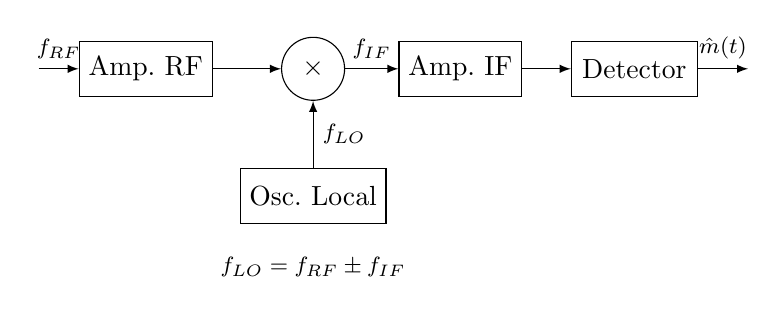
\begin{tikzpicture}[>=latex, scale=0.85]
\node[draw, rectangle, minimum width=1.5cm, minimum height=0.7cm] (rf) at (0,0) {Amp.\ RF};
\node[draw, circle, minimum size=0.8cm] (mix) at (2.5,0) {$\times$};
\node[draw, rectangle, minimum width=1.5cm, minimum height=0.7cm] (if) at (4.7,0) {Amp.\ IF};
\node[draw, rectangle, minimum width=1.6cm, minimum height=0.7cm] (det) at (7.3,0) {Detector};

\node[draw, rectangle, minimum width=1.6cm, minimum height=0.7cm] (lo) at (2.5,-1.9) {Osc.\ Local};

\draw[->] (-1.6,0) -- node[above, font=\footnotesize] {$f_{RF}$} (rf);
\draw[->] (rf) -- (mix.west);
\draw[->] (mix.east) -- node[above, font=\footnotesize] {$f_{IF}$} (if);
\draw[->] (if) -- (det);
\draw[->] (det) -- node[above, font=\footnotesize] {$\hat m(t)$} (9,0);
\draw[->] (lo.north) -- node[right, font=\footnotesize] {$f_{LO}$} (mix.south);

\node[below of=lo, node distance=0.9cm, font=\footnotesize] {$f_{LO} = f_{RF} \pm f_{IF}$};
\end{tikzpicture}
\end{center}

\small Amplificador RF sintonizado em torno do canal desejado; mixer translada para a IF; amplificador IF concentra ganho e seletividade; detector demodula.

\end{frame}

% ============================================

\begin{frame}{Vantagens do Superheterodino}

\textbf{Vantagens:}

\begin{enumerate}
\item \textbf{Seletividade:}
   \begin{itemize}
   \item Filtro IF fixo pode ser muito seletivo
   \item Não precisa ajustar filtro ao trocar estação
   \end{itemize}

\item \textbf{Sensibilidade:}
   \begin{itemize}
   \item Amplificação concentrada em frequência fixa
   \item Melhor controle de ganho (AGC)
   \end{itemize}

\item \textbf{Estabilidade do caminho IF:}
   \begin{itemize}
   \item Filtro IF, amp IF e demodulador operam em frequência fixa $\to$ deriva térmica e tolerâncias previsíveis e calibráveis
   \item O LO continua variável; sua estabilidade é tratada à parte (cristal, PLL, AFC)
   \end{itemize}
\end{enumerate}

\textbf{Próximo problema:} a mistura cria uma \textbf{frequência imagem} que precisa ser rejeitada antes do mixer.

\end{frame}

% ============================================

\begin{frame}{Exemplo: Receptor FM Superheterodino}

\textbf{Rádio FM comercial:}

\begin{itemize}
\item Banda FM: 88-108 MHz
\item IF padrão: $f_{IF} = 10.7$ MHz
\end{itemize}

\textbf{Para receber} $f_{RF} = 100.0$ MHz:

\[
f_{LO} = f_{RF} + f_{IF} = 100.0 + 10.7 = 110.7 \text{ MHz}
\]

\textbf{Frequência imagem:}
\[
f_{im} = f_{LO} + f_{IF} = 110.7 + 10.7 = 121.4 \text{ MHz}
\]

Fora da banda FM (88-108 MHz) $\rightarrow$ filtro RF facilmente rejeita

\end{frame}

% ============================================

\begin{frame}{Conversão superheterodina}

\begin{center}
\includegraphics[height=0.64\textheight,keepaspectratio]{figures/cap4/superheterodyne_conversion.pdf}
\end{center}

\end{frame}

% ============================================

\begin{frame}{O problema da frequência imagem}

\textbf{Receptor com} $f_{IF} = 10{,}7$\,MHz, $f_{LO} = 110{,}7$\,MHz. Sinal desejado em $f_d = 100$\,MHz; \textbf{imagem} em $f_i = f_{LO} + f_{IF} = 121{,}4$\,MHz.

\begin{center}
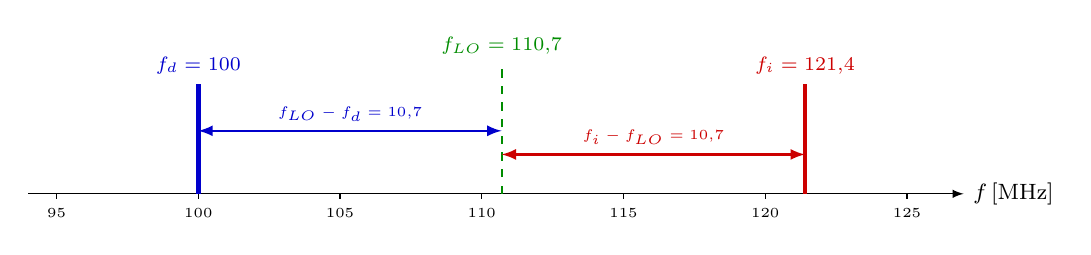
\begin{tikzpicture}[>=latex, x=0.36cm, y=0.5cm, every node/.style={font=\footnotesize}]
\draw[->] (-1,0) -- (32,0) node[right] {$f$\,[MHz]};
% Sinal desejado em 100 MHz (x = 5)
\draw[ultra thick, blue!80!black] (5,0) -- (5,2.8);
\node[blue!80!black, anchor=south, font=\scriptsize] at (5,2.8) {$f_d = 100$};
% LO em 110.7 MHz (x = 15.7)
\draw[thick, green!55!black, dashed] (15.7,0) -- (15.7,3.3);
\node[green!55!black, anchor=south, font=\scriptsize] at (15.7,3.3) {$f_{LO} = 110{,}7$};
% Imagem em 121.4 MHz (x = 26.4)
\draw[ultra thick, red!80!black] (26.4,0) -- (26.4,2.8);
\node[red!80!black, anchor=south, font=\scriptsize] at (26.4,2.8) {$f_i = 121{,}4$};
% Setas mostrando 10.7 MHz de cada lado de f_LO
\draw[<->, blue!80!black, thick] (5,1.6) -- (15.7,1.6);
\node[blue!80!black, anchor=south, font=\tiny] at (10.35,1.6) {$f_{LO}-f_d = 10{,}7$};
\draw[<->, red!80!black, thick] (15.7,1) -- (26.4,1);
\node[red!80!black, anchor=south, font=\tiny] at (21.05,1) {$f_i-f_{LO} = 10{,}7$};
% Ticks (95, 100, 105, ..., 125)
\foreach \k in {0,5,...,30} {
  \pgfmathtruncatemacro{\flab}{\k + 95}
  \draw (\k,0) -- (\k,-0.12);
  \node[anchor=north, font=\tiny] at (\k,-0.12) {\flab};
}
\end{tikzpicture}
\end{center}

\textbf{Após o mixer:} tanto $f_d$ quanto $f_i$ caem em $f_{IF} = 10{,}7$\,MHz e se somam, gerando interferência. \textbf{Filtro de RF antes do mixer} atenua $f_i$ preservando $f_d$.

\end{frame}

% ============================================

\begin{frame}{Como o filtro RF atua sobre a imagem}

\only<1>{\textbf{Sem filtro:} $f_d = 100$\,MHz e $f_i = 121{,}4$\,MHz chegam ambos ao mixer e colidem em $f_{IF}$.}
\only<2>{\textbf{Inserindo filtro RF:} passa-faixa largo cobrindo 88--108\,MHz da banda comercial.}
\only<3>{\textbf{Resultado:} $f_d$ está dentro da passagem (passa); $f_i$ está fora (atenuada).}

\begin{center}
\begin{tikzpicture}[>=latex, x=0.32cm, y=0.55cm, every node/.style={font=\footnotesize}]
\draw[->] (-1,0) -- (37,0) node[right] {$f$\,[MHz]};

% Filtro RF aparece a partir do estágio 2
\only<2->{
  \fill[green!12] plot[domain=-3.5:3.5, samples=80] (10+\x*3, {2.5/(1+(\x/2.5)^6)}) -- (21,0) -- (-1,0) -- cycle;
  \draw[thick, green!55!black] plot[domain=-3.5:3.5, samples=80] (10+\x*3, {2.5/(1+(\x/2.5)^6)});
  \node[green!55!black, anchor=south, font=\scriptsize] at (10,2.55) {filtro RF};
  \draw[<->, thick, green!55!black] (0,-0.55) -- (20,-0.55);
  \node[green!55!black, font=\tiny, anchor=north] at (10,-0.55) {$B_{RF} = 20$\,MHz};
}

% Sinal desejado em 100 MHz - sempre presente, altura cheia
\draw[ultra thick, blue!80!black] (12,0) -- (12,2.3);
\node[blue!80!black, anchor=south, font=\scriptsize] at (12,2.3) {$f_d = 100$};

% LO em 110.7 - sempre tracejado
\draw[thick, gray!40!black, dashed] (22.7,0) -- (22.7,1.6);
\node[gray!40!black, anchor=south, font=\tiny] at (22.7,1.6) {$f_{LO}$};

% Imagem em 121.4 - cheia nos estágios 1-2, atenuada no estágio 3
\only<1-2>{
  \draw[ultra thick, red!80!black] (33.4,0) -- (33.4,2.3);
  \node[red!80!black, anchor=south, font=\scriptsize] at (33.4,2.3) {$f_i = 121{,}4$};
}
\only<3>{
  \draw[ultra thick, red!80!black, dashed] (33.4,0) -- (33.4,2.3);
  \draw[ultra thick, red!80!black] (33.4,0) -- (33.4,0.3);
  \node[red!80!black, anchor=south, font=\scriptsize] at (33.4,2.3) {$f_i$ atenuada};
}

% Ticks sempre presentes
\foreach \x/\lab in {0/88, 12/100, 20/108, 33.4/121.4} {
  \draw (\x,0) -- (\x,-0.12);
  \node[anchor=north, font=\tiny] at (\x,-0.16) {\lab};
}
\end{tikzpicture}
\end{center}

\only<3>{
\textbf{Especificação do filtro RF:} rejeitar acima de 108\,MHz. A imagem está a $121{,}4 - 108 = 13{,}4$\,MHz da borda -- distância confortável.\quad
\textbf{$Q$ exigido:} $\sim f_c / 2 f_{IF} \approx 5$.

\textbf{Divisão de trabalho:} filtro RF (largo, $Q\sim 5$) cuida da imagem; filtro IF (estreito, $Q = 50$ em 10,7\,MHz) cuida da seleção de canal de 200\,kHz.
}

\end{frame}

% ============================================

\begin{frame}{Processamento no receptor FM}

\textbf{Processamento:}
\begin{itemize}
\item Amplificador RF sintonizado em 100 MHz
\item Mixer com LO de 110.7 MHz
\item Amplificador IF em 10.7 MHz (filtro muito seletivo)
\item Discriminador FM ou PLL para demodular
\end{itemize}

\end{frame}

% ============================================

\section{FDM}

\begin{frame}{Multiplexação em frequência}

\textbf{FDM (Frequency Division Multiplexing):}

Múltiplos sinais compartilham mesmo canal, cada um em frequência diferente.

\begin{center}
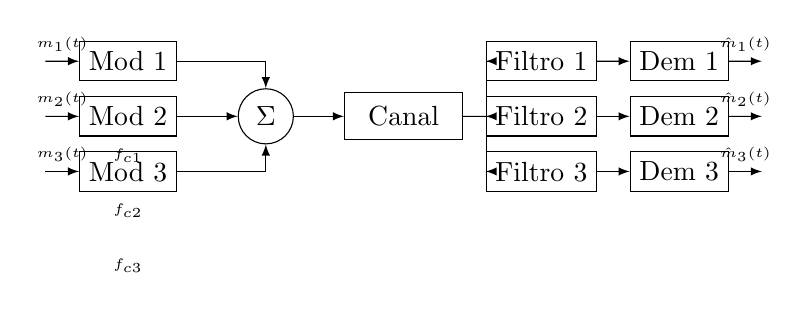
\begin{tikzpicture}[>=latex, scale=0.7]
% Transmissor
\node[draw, rectangle, minimum width=1.2cm, minimum height=0.5cm] (m1) at (0,2) {Mod 1};
\node[draw, rectangle, minimum width=1.2cm, minimum height=0.5cm] (m2) at (0,1) {Mod 2};
\node[draw, rectangle, minimum width=1.2cm, minimum height=0.5cm] (m3) at (0,0) {Mod 3};
\node[draw, circle, minimum size=0.7cm] (sum) at (2.5,1) {$\Sigma$};
\node[draw, rectangle, minimum width=1.5cm, minimum height=0.6cm] (canal) at (5,1) {Canal};

% Receptor
\node[draw, rectangle, minimum width=1.2cm, minimum height=0.5cm] (f1) at (7.5,2) {Filtro 1};
\node[draw, rectangle, minimum width=1.2cm, minimum height=0.5cm] (f2) at (7.5,1) {Filtro 2};
\node[draw, rectangle, minimum width=1.2cm, minimum height=0.5cm] (f3) at (7.5,0) {Filtro 3};
\node[draw, rectangle, minimum width=1.2cm, minimum height=0.5cm] (d1) at (10,2) {Dem 1};
\node[draw, rectangle, minimum width=1.2cm, minimum height=0.5cm] (d2) at (10,1) {Dem 2};
\node[draw, rectangle, minimum width=1.2cm, minimum height=0.5cm] (d3) at (10,0) {Dem 3};

% Conexões TX
\draw[->] (-1.5,2) -- node[above, font=\tiny] {$m_1(t)$} (m1);
\draw[->] (-1.5,1) -- node[above, font=\tiny] {$m_2(t)$} (m2);
\draw[->] (-1.5,0) -- node[above, font=\tiny] {$m_3(t)$} (m3);
\draw[->] (m1) -| (sum.north);
\draw[->] (m2) -- (sum.west);
\draw[->] (m3) -| (sum.south);
\draw[->] (sum) -- (canal);

% Conexões RX
\draw (canal.east) -- (6.5,1);
\draw[->] (6.5,1) |- (f1);
\draw[->] (6.5,1) -- (f2);
\draw[->] (6.5,1) |- (f3);
\draw[->] (f1) -- (d1);
\draw[->] (f2) -- (d2);
\draw[->] (f3) -- (d3);
\draw[->] (d1) -- node[above, font=\tiny] {$\hat{m}_1(t)$} (11.5,2);
\draw[->] (d2) -- node[above, font=\tiny] {$\hat{m}_2(t)$} (11.5,1);
\draw[->] (d3) -- node[above, font=\tiny] {$\hat{m}_3(t)$} (11.5,0);

% Portadoras
\node[below of=m1, node distance=1.2cm, font=\tiny] {$f_{c1}$};
\node[below of=m2, node distance=1.2cm, font=\tiny] {$f_{c2}$};
\node[below of=m3, node distance=1.2cm, font=\tiny] {$f_{c3}$};
\end{tikzpicture}
\end{center}

\textbf{Requisito:} $f_{ci}$ suficientemente espaçadas para evitar sobreposição espectral

\textbf{Aplicações:} TV a cabo, telefonia analógica (hierarquia FDM)

\end{frame}

% ============================================

\begin{frame}{Exemplo: FDM em Telefonia}

\textbf{Hierarquia FDM analógica (histórica):}

\begin{itemize}
\item \textbf{Grupo:} 12 canais de voz (4 kHz cada)
  \begin{itemize}
  \item SSB-LSB, espaçamento de 4 kHz
  \item Faixa: 60-108 kHz
  \item Banda total: 48 kHz
  \end{itemize}

\item \textbf{Supergrupo:} 5 grupos = 60 canais
  \begin{itemize}
  \item Faixa: 312-552 kHz
  \item Banda: 240 kHz
  \end{itemize}

\item \textbf{Grupo mestre:} 10 supergrupos = 600 canais
  \begin{itemize}
  \item Faixa: 564-3084 kHz
  \item Banda: 2520 kHz
  \end{itemize}
\end{itemize}

\vspace{0.3cm}

\textbf{Nota:} Substituído por sistemas digitais (TDM, SONET/SDH), mas princípio permanece em sistemas ópticos (WDM).

\end{frame}

% ============================================

\begin{frame}{Resumo: FM vs.\ PM e Espectro}

\textbf{FM vs. PM:}
\begin{itemize}\itemsep0pt
\item FM -- frequência $\propto m(t)$, fase $\propto \int m(t)$. Mais comum, melhor em ruído.
\item PM -- fase $\propto m(t)$, frequência $\propto dm(t)/dt$.
\end{itemize}

\vspace{0.3cm}
\textbf{Espectro FM:}
\begin{itemize}\itemsep0pt
\item Infinitas bandas laterais via Bessel.
\item Carson: $B \approx 2(\Delta f + f_m)$.
\item NBFM se $\beta \ll 1$; WBFM se $\beta \gg 1$.
\end{itemize}

\end{frame}

% ============================================

\begin{frame}{Resumo: Demodulação e Geração}

\textbf{Demodulação:}
\begin{itemize}\itemsep0pt
\item Discriminador de frequência -- precisa de limitador antes para rejeitar ruído de amplitude.
\item PLL -- mais usado atualmente, intrinsecamente imune a variações de amplitude.
\end{itemize}

\vspace{0.3cm}
\textbf{Geração:}
\begin{itemize}\itemsep0pt
\item Direta -- VCO, simples mas instável em $f_c$.
\item Indireta -- método de Armstrong, NBFM com cristal seguido de multiplicação.
\end{itemize}

\vspace{0.3cm}
\textbf{Receptor:}
\begin{itemize}\itemsep0pt
\item Arquitetura superheterodina, IF fixa de 10,7\,MHz no caso comercial.
\end{itemize}

\end{frame}
